%! TeX program = lualatex
\documentclass[12pt,a4paper]{report}
\usepackage{dissertation}
\makeglossaries
\makeindex

\logo{EE}{Escola de Engenharia}{}
\logoB{EE}{Escola de Engenharia}{}

\author{Tiago Passos Rodrigues}

\titleA{Um sistema para registo seguro do}
\titleB{consentimento de processamento}
\titleC{de dados pessoais}

\masters{Mestrado em Engenharia Informática}
%\area{Área de especialização}
\supervisor{João Marco Cardoso da Silva}
\cosupervisor{Ana Luísa Parreira Nunes Alonso}

\bibpunct[,]{(}{)}{;}{a}{,}{,}
\begin{document}
\setlength{\parindent}{0em}

%-- Covers
\begin{titlepage}
\color{PANTONECoolGray7C}
\thelogo
\leading{20.4pt}
{\Large
\theauthor
\\
%
\\
\textbf{\thetitleA}
\\
\textbf{\thetitleB}
\\
\textbf{\thetitleC}
}

\vspace*{\fill}
{\footnotesize \myear}
\end{titlepage}

\null
\thispagestyle{empty}
\pagecolor{PANTONECoolGray7C}
\afterpage{\nopagecolor}
\newpage

\begin{titlepage}
\color{PANTONECoolGray7C}
\thelogoB
\leading{20.4pt}
{\Large
\theauthor
\\
%
\\
\textbf{\thetitleA}
\\
\textbf{\thetitleB}
\\
\textbf{\thetitleC}
}

\vspace{55.2mm}
\leading{16.8pt}
{\large
Dissertação de Mestrado
\\
\themasters
\\
\thearea
Trabalho efetuado sob a orientação de
\\
\textbf{\thesupervisor}
\\
\thecosupervisor}

\vspace*{\fill}
{\footnotesize \myear}
\end{titlepage}

%-- Document setup
\newgeometry{right=25mm, left=25mm, top=25mm, bottom=25mm}
\pagenumbering{roman}

\setlength{\parskip}{0pt}
\setlength{\parindent}{1.5em}

%-- Preamble
\chapter*{Direitos de Autor e Condições de Utilização do Trabalho por Terceiros}
\setlength{\parskip}{1em}
\noindent
Este é um trabalho académico que pode ser utilizado por terceiros desde que respeitadas as regras e boas práticas internacionalmente aceites, no que concerne aos direitos de autor e direitos conexos.

\noindent
Assim, o presente trabalho pode ser utilizado nos termos previstos na licença abaixo indicada.

\noindent
Caso o utilizador necessite de permissão para poder fazer um uso do trabalho em condições não previstas no licenciamento indicado, deverá contactar o autor, através do RepositóriUM da Universidade do Minho.

\section*{Licença concedida aos utilizadores deste trabalho:}

\textit{[Caso o autor pretenda usar uma das licenças Creative Commons, deve escolher e deixar apenas um dos seguintes ícones e respetivo lettering e URL, eliminando o texto em itálico que se lhe segue. Contudo, é possível optar por outro tipo de licença, devendo, nesse caso, ser incluída a informação necessária adaptando devidamente esta minuta]}

\noindent

\includegraphics[]{images/CCBY.png}
\\
\textbf{CC BY}
\\
\url{https://creativecommons.org/licenses/by/4.0/}
\textit{[Esta licença permite que outros distribuam, remixem, adaptem e criem a partir do seu trabalho, mesmo para fins comerciais, desde que lhe atribuam o devido crédito pela criação original. É a licença mais flexível de todas as licenças disponíveis. É recomendada para maximizar a disseminação e uso dos materiais licenciados.]}

%--

\noindent

\includegraphics[]{images/CCBYSA.png}
\\
\textbf{CC BY-SA}
\\
\url{https://creativecommons.org/licenses/by-sa/4.0/}
\textit{[Esta licença permite que outros remisturem, adaptem e criem a partir do seu trabalho, mesmo para fins comerciais, desde que lhe atribuam o devido crédito e que licenciem as novas criações ao abrigo de termos idênticos. Esta licença costuma ser comparada com as licenças de software livre e de código aberto «copyleft». Todos os trabalhos novos baseados no seu terão a mesma licença, portanto quaisquer trabalhos derivados também permitirão o uso comercial. Esta é a licença usada pela Wikipédia e é recomendada para materiais que seriam beneficiados com a incorporação de conteúdos da Wikipédia e de outros projetos com licenciamento semelhante.]}

%--

\noindent

\includegraphics[]{images/CCBYND.png}
\\
\textbf{CC BY-ND}
\\
\url{https://creativecommons.org/licenses/by-nd/4.0/}
\textit{[Esta licença permite que outras pessoas usem o seu trabalho para qualquer fim, incluindo para fins comerciais. Contudo, o trabalho, na forma adaptada, não poderá ser partilhado com outras pessoas e têm que lhe ser atribuídos os devidos créditos.]}

%--

\noindent

\includegraphics[]{images/CCBYNC.png}
\\
\textbf{CC BY-NC}
\\
\url{https://creativecommons.org/licenses/by-nc/4.0/}
\textit{[Esta licença permite que outros remisturem, adaptem e criem a partir do seu trabalho para fins não comerciais, e embora os novos trabalhos tenham de lhe atribuir o devido crédito e não possam ser usados para fins comerciais, eles não têm de licenciar esses trabalhos derivados ao abrigo dos mesmos termos.]}

%--

\noindent

\includegraphics[]{images/CCBYNCSA.png}
\\
\textbf{CC BY-NC-SA}
\\
\url{https://creativecommons.org/licenses/by-nc-sa/4.0/}
\textit{[Esta licença permite que outros remisturem, adaptem e criem a partir do seu trabalho para fins não comerciais, desde que lhe atribuam a si o devido crédito e que licenciem as novas criações ao abrigo de termos idênticos.]}

%--

\noindent

\includegraphics[]{images/CCBYNCND.png}
\\
\textbf{CC BY-NC-ND}
\\
\url{https://creativecommons.org/licenses/by-nc-nd/4.0/}
\textit{[Esta é a mais restritiva das nossas seis licenças principais, só permitindo que outros façam download dos seus trabalhos e os compartilhem desde que lhe sejam atribuídos a si os devidos créditos, mas sem que possam alterá- los de nenhuma forma ou utilizá-los para fins comerciais.]}

\setlength{\parskip}{0em}
\chapter*{Agradecimentos}
\setlength{\parskip}{1em}

Escreva aqui os seus agradecimentos. Não se esqueça de mencionar, caso seja esse o caso, os projetos e bolsas dos quais se beneficiou enquanto fazia a sua investigação. Pergunte ao seu orientador sobre o formato específico a ser usado. (As agências de financiamento são bastante rigorosas quanto a isso.)

\setlength{\parskip}{0em}
\chapter*{Declaração de Integridade}
\setlength{\parskip}{1em}
\noindent
Declaro ter atuado com integridade na elaboração do presente trabalho académico e confirmo que não recorri à prática de plágio nem a qualquer forma de utilização indevida ou falsificação de informações ou resultados em nenhuma das etapas conducente à sua elaboração.

\noindent
Mais declaro que conheço e que respeitei o Código de Conduta Ética da Universidade do Minho.


\phantom{space for signature}

\noindent
Universidade do Minho, Braga, \myear

\vspace{25mm}
\noindent\theauthor
\setlength{\parskip}{0em}
\chapter*{Resumo}

% O que se quer no resumo então?

%Escrever aqui o resumo (pt)
A proteção da privacidade dos utilizadores tornou-se cada vez mais complexo com a crescente recolha de dados pessoais e a exigência de conformidade com regulamentos como o \acrfull{rgpd}.
Embora existam plataformas para gerir consentimentos, estas não oferecem ao utilizador uma forma clara de comprovar se as suas escolhas foram respeitadas.

Esta dissertação propõe uma abordagem que permite registar consentimentos de forma verificável e imutável, criando evidências que podem ser usadas como prova em caso de incumprimento.
O sistema desenvolvido gera registos que garantem integridade e não repúdio, permitindo ao utilizador demonstrar as suas escolhas.
Os testes realizados demonstraram que é possível gerar registos fiáveis, capazes de sustentar disputas e aumentar a autonomia do utilizador.

Este trabalho apresenta uma solução prática que abre caminho para evoluções futuras orientadas para maior controlo e confiança na gestão de consentimento.

\paragraph{Palavras-chave} consentimento, \acrshort{cmp}, \acrshort{rgpd}, transparência, privacidade
% Demasiado genericos, rever

\cleardoublepage

\chapter*{Abstract}

%Write abstract here (en)
Protecting user privacy has become a central challenge with the growing collection of personal data and the need to comply with regulations such as \acrfull{gdpr}.
Existing consent management platforms allow users to express their preferences but do not provide a clear way for them to verify whether those choices were respected.

This dissertation proposes an approach that records consent in a verifiable and immutable manner, creating evidence that can be used as proof in cases of non-compliance.
The developed system generates records that ensure integrity and non-repudiation, allowing users to demonstrate their choices.
Tests have shown that it is possible to produce reliable records capable of supporting disputes and increasing user autonomy.

This work proposes a practical solution that opens the door to future developments aimed at greater control and confidence in consent management.

\paragraph{Keywords} consent, \acrshort{cmp}, \acrshort{gdpr}, transparency, privacy
\cleardoublepage


\phantomsection
\tableofcontents

\cleardoublepage
\listoffigures

% List of tables
\listoftables
\clearpage

% garantir que definicao de acronomimos aparecem na primeira vez

\newacronym{rgpd}{RGPD}{Regulamento Geral de Proteção de Dados}

\newacronym{cmp}{CMP}{Plataformas de Gestão de Consentimento}

\newacronym{gdpr}{GDPR}{\textit{General Data Protection Regulation}}

\newacronym{ue}{UE}{União Europeia}

\newacronym{eda}{EA}{Estado da Arte}

\newacronym{ds}{DS}{\textit{Data Subject}}
\newacronym{dc}{DC}{\textit{Data Controller}}
\newacronym{dr}{DR}{\textit{Data Recipient}}
\newacronym{dp}{DP}{\textit{Data Processor}}
\newacronym{sp}{SP}{\textit{Service Provider}}

\newacronym{api}{API}{\textit{Application Programming Interface}}

\newacronym{ca}{CA}{\textit{Certificate Authority}}

\newacronym{ccpa}{CCPA}{\textit{California Privacy Rights Act}}

\newacronym{jws}{JWS}{\textit{JSON Web Signatures}}

% Acronyms
\printglossary[type=\acronymtype,nonumberlist, title={Acrónimos}]

% Glossary
\printglossary[title={Glossário}, nonumberlist]

\cleardoublepage
\pagenumbering{arabic}

%-- Dissertation 
%\part{Material Introdutório}

\chapter{Introdução}

%Contexto, motivação, principais objetivos.

\section{Contextualização}

Com a digitalização em crescimento e a utilização crescente de plataformas online, a quantidade de dados pessoais recolhidos dos utilizadores tem aumentado exponencialmente. Contudo, muitos utilizadores desconhecem como esses dados são recolhidos, processados e partilhados pelos servidores. Quando um utilizador acede a um site, ele frequentemente não tem uma visão clara sobre o que acontece com os dados fornecidos nem se o servidor recebeu exatamente aquilo a que deu consentimento. Este cenário levanta questões de privacidade, especialmente no que diz respeito ao cumprimento de regulamentações como o \acrfull{rgpd} e outras legislações de privacidade.

No contexto atual, as Plataformas de Gestão de Consentimento (\acrshort{cmp}s) surgem como ferramentas que dizem assegurar às plataformas das empresas que assim podem cumprir o \acrshort{rgpd} \citep{Santos2021}, permitindo a recolha e gestão do consentimento dos utilizadores para a utilização dos seus dados. Contudo, as \acrshort{cmp}s tradicionais, muitas das quais são soluções fechadas, apresentam limitações em termos de transparência e auditoria. Estas plataformas não fornecem uma visão clara sobre o que realmente acontece com os dados depois de o utilizador ter dado o seu consentimento, nem se a informação transmitida ao servidor está em conformidade com a escolha do utilizador. A falta de uma auditoria transparente torna difícil garantir que as empresas estão a respeitar o consentimento dos utilizadores e a cumprir as regulamentações de privacidade.

\section{Motivação}

A motivação para este projeto surge precisamente da necessidade de permitir a auditoria desse fluxo de dados, oferecendo uma forma de garantir que as escolhas do utilizador são efetivamente respeitadas. Uma das grandes limitações das \acrshort{cmp}s tradicionais é o facto de muitas delas serem soluções fechadas, dificultando a compreensão e auditoria do que acontece com os dados. Por isso, optou-se por explorar soluções de \acrshort{cmp} \textit{open source}, que, ao serem mais acessíveis, permitem uma maior transparência e auditabilidade dos dados recolhidos. Através dessas plataformas, é possível compreender melhor os fluxos de dados e garantir que o processo de consentimento seja claro e auditável.

\section{Objetivos}

O objetivo deste trabalho é criar uma solução que permita não só recolher e gerir o consentimento dos utilizadores, mas também auditar o processo de forma transparente e verificável. Uma possível solução para isso é o uso de tecnologias como \textit{blockchain}, que, ao permitir registar de forma imutável as interações e escolhas dos utilizadores, pode assegurar a conformidade e aumentar a confiança no processo. O principal objetivo deste trabalho é, portanto, desenhar e prototipar um sistema que ajuda na gestão do consentimento do utilizador uma vez que se integra a recolha de consentimento com mecanismos de auditoria transparentes, utilizando tecnologias como \textit{blockchain}, de forma a criar transparência entre as decisões dos utilizadores e os dados que são armazenados nas \acrshort{cmp} e que esteja conforme o \acrshort{rgpd}.

Para atingir este objetivo, será realizada inicialmente uma revisão de literatura sobre \acrshort{cmp}s, \acrshort{rgpd} e a utilização de \textit{blockchain} para auditoria de consentimento e integração de contratos inteligentes. Em seguida, proceder-se-á à análise das abordagens existentes para plataformas de gestão de consentimento, identificando as suas limitações e as melhores alternativas para o nosso sistema. Com base nesta análise, será desenhado um modelo arquitetural para uma plataforma que integre auditoria transparente e registo imutável de consentimentos atráves de uma rede de \textit{blockchain} (ex. Ethereum). Posteriormente, será desenvolvido um protótipo funcional da solução proposta, garantindo a integração entre a \acrshort{cmp} e um registo \textit{blockchain}. O sistema será testado e otimizado, avaliando-se o seu desempenho, segurança e usabilidade.

\section{Estrutura da dissertação}



\chapter{Trabalho Relacionado}
\label{cap:relacionado}

%Estado da arte revisto; trabalho relacionado.
A gestão de consentimento é um dos principais desafios no tratamento de dados pessoais, especialmente face ao crescimento exponencial da digitalização e às regulamentações como o \acrshort{rgpd} \citep{gdpr}.
As \acrshort{cmp}s surgem como uma solução prática para facilitar a recolha e a gestão do consentimento do utilizador com vista a assegurar a conformidade com esta legislação. No entanto, apesar das \acrshort{cmp}s oferecerem mecanismos para gerir o consentimento, existem limitações em termos de transparência e auditabilidade.

\section{\acrfull{rgpd}}

O \acrshort{rgpd} é o instrumento legislativo da \acrfull{ue} que define as regras relativas à proteção das pessoas singulares no que respeita ao tratamento de dados pessoais e à livre circulação desses dados. Reconhecendo que a proteção de dados pessoais constitui um direito fundamental, o \acrshort{rgpd} visa harmonizar as legislações dos Estados-Membros, garantindo a privacidade dos cidadãos e permitindo, dentro desse quadro, a circulação segura e legal de dados no mercado interno da União Europeia.

Além de estabelecer normas rigorosas para o tratamento de dados, o \acrshort{rgpd} reforça os direitos dos titulares dos dados, incluindo o direito de acesso, retificação, remoção (direito a ser esquecido), portabilidade, limitação do tratamento e oposição. As organizações são também obrigadas a obter o consentimento explícito e informado dos utilizadores para o processamento dos seus dados pessoais. \citep{Daudén-Esmel2024}

O \acrshort{rgpd} identifica quatro intervenientes principais no seu quadro legal \citep{gdpr2016}:  
\begin{itemize}
    \item \textit{Titular dos Dados} (\textit{Data Subject} (\acrshort{ds})): A pessoa natural identificada ou identificável de quem as entidades podem recolher informações pessoais.  
    \item \textit{Responsável pelo Tratamento} (\textit{Data Controller} (\acrshort{dc})): A pessoa natural ou entidade legal que determina as finalidades e os meios pelos quais os dados pessoais são processados.  
    \item \textit{Destinatário dos Dados} (\textit{Data Recipient} (\acrshort{dr})): A pessoa natural ou entidade legal para a qual os dados pessoais são divulgados (pode ser o próprio \acrshort{dc} ou um terceiro).  
    \item \textit{Subcontratante} (\textit{Data Processor} (\acrshort{dp})): A pessoa natural ou entidade legal que processa dados pessoais em nome do \acrshort{dc}.
\end{itemize}

O principal objetivo do \acrshort{rgpd} é garantir direitos de privacidade específicos aos titulares dos dados, assegurando que os seus dados pessoais “só podem ser recolhidos legalmente, sob condições estritas e para um propósito legítimo”. O regulamento procura devolver o controlo total sobre os dados aos seus titulares. Adicionalmente, o \acrshort{rgpd} trouxe benefícios relevantes, como o aumento da consciência sobre a segurança e proteção de dados e a capacitação dos consumidores para controlar as suas preferências e participar ativamente na preservação dos seus direitos.

A conformidade com o \acrshort{rgpd} é obrigatória para todas as organizações que tratem dados de cidadãos da \acrshort{ue}, independentemente da sua localização geográfica. A não conformidade pode resultar em sanções severas, o que tem impulsionado o desenvolvimento de ferramentas como as \acrshort{cmp}s. Estas plataformas ajudam as organizações a cumprir os requisitos legais impostos por este regulamento, mas frequentemente enfrentam limitações em termos de transparência e auditabilidade (\cite{ribeiro2025assessing}, \cite{ramos2019privacy}).

Por fim, uma das características mais relevantes do \acrshort{rgpd} é o seu enfoque na responsabilização e transparência no tratamento de dados pessoais. O regulamento exige que os \acrfull{sp} sejam capazes de demonstrar a conformidade com as disposições legais e de documentar os acordos estabelecidos com os \textit{titulares dos dados}. Este princípio de responsabilização reforça a importância de adotar abordagens inovadoras e ferramentas tecnológicas que promovam maior confiança, rastreabilidade e conformidade com as normas regulamentares.

\newpage

\section{\texorpdfstring{\acrfull{cmp}}{CMP}}

As \acrfull{cmp} têm como objetivo central gerir o consentimento dos \textit{titulares dos dados} de forma clara, explícita e conforme às exigências legais de privacidade, como as do \acrshort{rgpd}. Estas plataformas permitem que os utilizadores definam as suas preferências relativamente à recolha e utilização dos seus dados pessoais, assegurando que as organizações apenas procedem ao tratamento dentro dos limites autorizados. 

Uma \acrshort{cmp} funciona como um intermediário entre o utilizador e os serviços que recolhem ou processam dados. Apresenta as finalidades do tratamento, recolhe e armazena as preferências expressas e comunica essas decisões aos sistemas envolvidos. Além de facilitar o cumprimento das obrigações legais, estas plataformas promovem transparência e reforçam a confiança dos utilizadores, ao garantirem maior controlo sobre o uso das suas informações pessoais.

\subsection{\acrshort{cmp} Open-Source}

A recolha de consentimentos do lado do servidor apresenta desafios significativos, tanto em termos de arquitetura como de conformidade regulatória. Este problema é exacerbado pelo facto de que a maioria das soluções de \acrshort{cmp} disponíveis são proprietárias, limitando a transparência e dificultando a auditabilidade das ferramentas.

As plataformas fechadas não permitem compreender facilmente como os dados são processados e armazenados após o consentimento. Esta falta de visibilidade cria barreiras à adoção de práticas verdadeiramente transparentes, essenciais para assegurar conformidade com regulamentações como o \acrshort{rgpd}
Os \acrshort{cmp}s \textit{open-source} oferecem maior flexibilidade e transparência, permitindo que as organizações compreendam e adaptem o funcionamento interno da ferramenta. Isto garante que os consentimentos são armazenados de forma consistente e auditável, favorece a confiança do utilizador, promove conformidade regulatória e facilita a integração com diferentes serviços e fluxos de recolha de dados.

\subsection{Fluxo de implementação de uma \acrshort{cmp}}

O fluxo típico para um \textit{provedor de serviços} apresentar ao utilizador as opções de consentimento, de acordo com os regulamentos, pode ser representado no diagrama de atividades da Figura~\ref{fig:diagrama-cmp}.
Este diagrama ilustra de forma genérica a integração de uma \acrshort{cmp} num website.
No âmbito da pesquisa realizada sobre soluções existentes, este fluxo foi exemplificado com a plataforma CookieChimp, utilizada apenas para efeitos de análise comparativa.

\begin{figure}
\begin{center}
    \begin{tikzpicture}[node distance=2cm]

        \node (A) [inicio] {Desenvolvedor cria um website};
        \node (B) [processo, below of=A] {Integra \acrshort{cmp} (ex: CookieChimp)};
        \node (C) [processo, below of=B] {Configura \acrshort{cmp} e adiciona JavaScript};
        \node (D) [inicio, below of=C] {Utilizador acessa site};
        \node (E) [processo, below of=D] {\acrshort{cmp} exibe banner de consentimento};
        \node (F) [decisao, below of=E, yshift=-1cm] {Utilizador decide};

        \node (G1) [processo, right of=F, xshift=4cm] {Aceita todos os \textit{cookies}};
        \node (G2) [processo, below of=F, yshift=-1cm] {Recusa \textit{cookies} não essenciais};
        \node (G3) [processo, left of=F, xshift=-4cm] {Personaliza preferências};

        \node (H) [processo, below of=G2] {\acrshort{cmp} armazena preferências};
        \node (J) [processo, below of=H] {Decisão registada (\textit{Dashboard} CookieChimp)};
        \node (K) [processo, below of=J] {Utilizador pode alterar preferências};

        % Conexões
        \draw [seta] (A) -- (B);
        \draw [seta] (B) -- (C);
        \draw [seta] (C) -- (D);
        \draw [seta] (D) -- (E);
        \draw [seta] (E) -- (F);
        \draw [seta] (F) -- (G1) node[midway, above] {Aceita tudo};
        \draw [seta] (F) -- (G2) node[midway, right] {Recusa};
        \draw [seta] (F) -- (G3) node[midway, above] {Personaliza};
        \draw [seta] (G1.south) |- (H);
        \draw [seta] (G2) -- (H);
        \draw [seta] (G3.south) |- (H);
        \draw [seta] (H) -- (J);
        \draw [seta] (J) -- (K) node[midway, right] {Se desejar};
    \end{tikzpicture}
\end{center}
    \caption{Fluxo de implementação de uma \acrshort{cmp} numa página web.}
\label{fig:diagrama-cmp}
\end{figure}

\newpage

O processo pode ser descrito da seguinte forma, detalhando os passos e as suas implicações:

\begin{enumerate}
    \item O desenvolvedor cria um site e identifica a necessidade de conformidade: o primeiro passo no ciclo de vida do projeto web é a sua conceção e implementação. É nesta fase inicial que o desenvolvedor mapeia as cookies necessárias e tecnologias de rastreamento utilizadas (próprias e de terceiros) para determinar o nível de risco e as obrigações regulamentares (ex: \acrshort{rgpd}, \acrfull{ccpa}).
    \item Integração e Escolha da \acrshort{cmp}: para cumprir os requisitos legais de obtenção de consentimento, o desenvolvedor decide integrar uma \acrshort{cmp}, como o CookieChimp.
    \item Configuração da \acrshort{cmp} e Adição do JavaScript: após a escolha, o desenvolvedor configura a ferramenta para o seu domínio (definindo políticas, idioma, e aspeto do \textit{banner}). O passo mais importante é a inserção de um pequeno código JavaScript fornecido pela \acrshort{cmp} no cabeçalho (\textit{header}) do site. Este \textit{script} é o responsável por carregar o \textit{banner}.
    \item Acesso do Utilizador e Exibição do Banner: quando um utilizador acessa o site, o \textit{script} da \acrshort{cmp} é o primeiro a ser executado, exibindo imediatamente um \textit{banner} (figura \ref{fig:banner}) solicitando o consentimento.
    \item Decisão do Utilizador: o utilizador tem controlo sobre a sua decisão, podendo:

    \begin{itemize}
        \item Aceitar todos os cookies e tecnologias de rastreamento.
        \item Recusar cookies não essenciais: a \acrshort{cmp} exige que cookies estritamente necessários para o funcionamento básico do site (como \textit{tokens} de sessões) sejam carregados. Todos os de marketing, estatísticas ou personalização permanecem bloqueados.
        \item Personalizar as suas preferências: o utilizador pode ligar/desligar categorias específicas de cookies (ex: marketing, estatísticas).
    \end{itemize}
    \item Armazenamento de Preferências e Bloqueio de Cookies: independentemente da escolha, a \acrshort{cmp} armazena a decisão numa cookie do lado do cliente com uma referência com a qual o servidor do CookieChimp interage de maneira a conseguir obter informação dos consentimentos guardados. Esta cookie serve como prova de consentimento e evita que o \textit{banner} seja exibido novamente nas visitas subsequentes durante o período de validade do consentimento (ex: 6 ou 12 meses).
    \item Registo da Decisão (Proof of Consent): a decisão detalhada do utilizador, a data e hora do consentimento são registadas e enviadas para o CookieChimp e pode ser acedido através do \textit{dashboard} do \textit{provedor de serviço}, como pode ser visto na figura \ref{fig:dashboard-visualizacao}.
    \item Alteração de Preferências: Para cumprir o princípio de que o consentimento deve ser tão fácil de retirar quanto de dar, o utilizador pode alterar as suas preferências a qualquer momento. Isto é geralmente realizado através de um botão ou link discreto, mas acessível (ex: um ícone flutuante ou link no rodapé), que reabre o \textit{banner} do \acrshort{cmp}.
\end{enumerate}


\begin{figure}[h]
    \begin{center}
	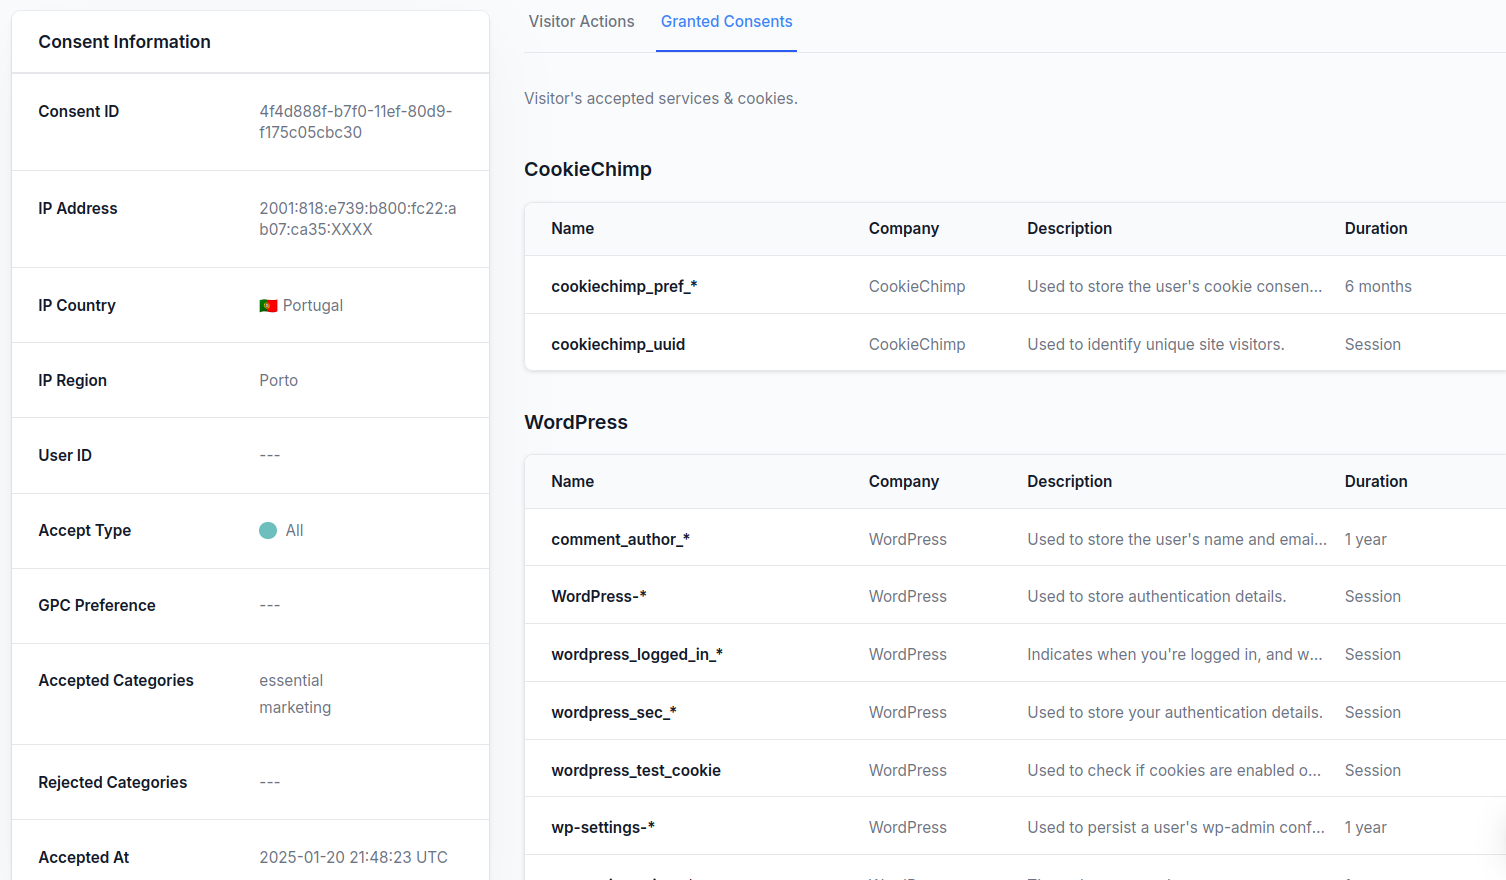
\includegraphics[width=1.0\textwidth]{images/consent.png}
    \end{center}
    \caption{Exemplo de visualização do consentimento na \textit{dashboard} do CookieChimp.}
\label{fig:dashboard-visualizacao}
\end{figure}

Desta forma, as \acrshort{cmp}s transmitem transparência e conformidade com as regulamentações de privacidade aos \textit{provedores de serviço}, e permitem que os utilizadores tenham escolha sobre os dados pessoais a partilhar.

\begin{figure}[h]
\begin{center}
	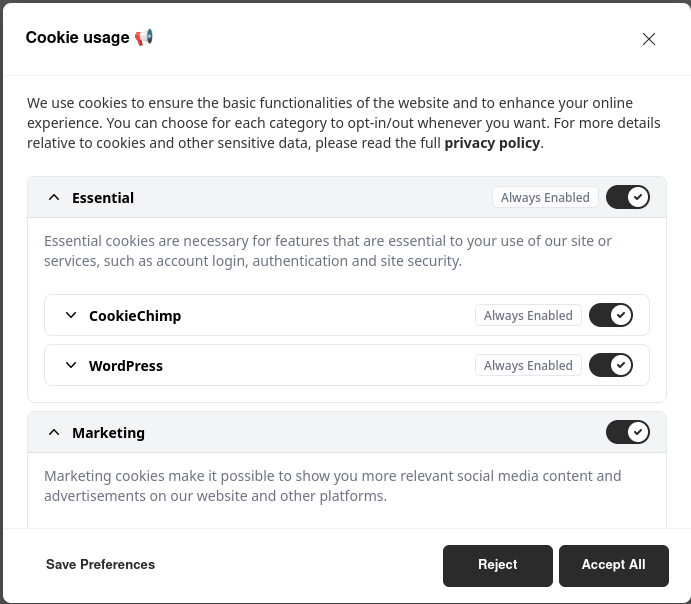
\includegraphics[width=1.0\textwidth]{images/banner.png}
\end{center}
\caption{Exemplo de banner de consentimento exibido ao utilizador.}
\label{fig:banner}
\end{figure}
% Tenho alguma duvida sobre a utilidade da figura

\newpage

\section{Plataformas e funcionalidades}
Entre as soluções encontra-se plataformas como Osano, Cookiebot, Tarteaucitron.js, Klaro.js e Consent Manager. Cada plataforma oferece funcionalidades específicas, mas têm em comum o foco na conformidade com as regulamentações de privacidade existentes.

\begin{itemize}
    \item Osano: Oferece uma interface intuitiva de personalização e um sistema eficiente de gestão de preferências, facilitadas por uma boa acessibilidade \cite{osano}. Inclui recursos avançados como armazenamento local de preferências, do lado do cliente, onde todo o acesso ao \textit{local storage} e aos \textit{cookies} (pequenos ficheiros de texto armazenados no navegador que guardam informações sobre as preferências e atividades do utilizador num site) feito pelo \textit{script} do Osano ocorre no contexto da página de execução e é tratado como \textit{cookie} de primeira parte. Isto significa que os dados do consentimento não são enviados a cada requisição, mas sim guardados localmente no \textit{browser}, utilizando o \textit{local storage} do navegador para armazenar dados auxiliares. Contudo, por ser uma solução proprietária, apresenta limitações na verificação do processamento de dados entre o navegador e o servidor, como por exemplo, opções limitadas de personalização, problemas de complexidade, exigindo suporte adicional para obter uma utilização mais eficaz para organizações de maiores dimensões e a gestão de cookies requer modificações extensas, tornando desafiador alcançar as funcionalidades desejadas.

    \item Cookiebot: Fornece uma solução robusta que analisa automaticamente até 10.000 páginas por domínio \cite{Cookiebot2024}. Implementa um sistema inteligente para detetar mudanças nos \textit{cookies} e rastreadores do website. O estado de consentimento do utilizador é armazenado localmente no navegador mediante um \textit{cookie}, denominado por \textit{CookieConsent}, que inclui um identificador único de consentimento (Consent ID) que se liga a um registo no servidor do Cookiebot para efeitos de auditoria da própria \acrshort{cmp} e prova legal. A principal limitação está na natureza fechada do código, que dificulta verificações independentes do funcionamento interno e a falta de possibilidade de auditoria do lado do cliente.

    \item Tarteaucitron.js \& Klaro.js: São soluções de código aberto que se destacam pela flexibilidade \cite{tarteaucitron}. Tarteaucitron.js permite extensões personalizadas e um carregamento otimizado de \textit{scripts} (fragmentos de código executados no navegador que permitem carregar funcionalidades externas, podendo recolher dados sobre a navegação do utilizador), armazenando as preferências de consentimento num \textit{cookie} do lado do cliente. Klaro.js oferece um sistema flexível de armazenamento de preferências e suporte a múltiplos idiomas, garantindo persistência local do lado do cliente sem necessidade de servidores externos. Ambos permitem personalização completa do controlo de \textit{cookies} e asseguram ser a ferramenta para estar em conformidade com os regulamentos impostos.

    \item Consent Manager: Permite sincronização instantânea das preferências do utilizador entre diferentes \textit{tabs} do navegador \cite{ConsentManager2024}. As preferências de consentimento são armazenadas localmente no navegador, assegurando a persistência das escolhas, sem necessidade de comunicação constante com o servidor. Embora ofereça recursos de gestão e uma integração eficiente, devido à sua natureza fechada, limita a transparência e dificulta a possibilidade de auditorias independentes de verificação do modo como os dados de consentimento são processados e como o sistema implementa o bloqueio e a transmissão de \textit{cookies} e rastreadores.

    \item CookieChimp: Destaca-se pela facilidade de integração com sistemas externos, como plataformas de análise, gestão de conteúdos e aplicações corporativas \cite{CookieChimp2024}. Disponibiliza uma \acrshort{api} RESTful, bem documentada, que permite a interoperabilidade com diferentes ambientes tecnológicos. A sua eficiência manifesta-se na capacidade de processar e sincronizar preferências de consentimento em tempo real, com baixo impacto no desempenho do website e elevada fiabilidade na atualização dos estados de consentimento.
\end{itemize}

Apesar dessas soluções estarem bem posicionadas para garantir a conformidade legal, um problema recorrente nas \acrshort{cmp}s existentes é a falta de visibilidade sobre os consentimentos transmitidos. Os utilizadores não sabem exatamente o que acontece com as suas informações durante a navegação, como os identificadores de sessão e preferências de consentimento, depois deste ser fornecido. Não existe uma forma clara e acessível para verificar se as escolhas feitas são efetivamente respeitadas, o que levanta questões sobre a transparência e a auditoria. Com isto em mente, nenhum dos \acrshort{cmp} oferece a possibilidade de o cliente poder demonstrar de forma independente as suas escolhas em termos de consentimento de uma maneira não repudiável e verificável, caso se torne evidente uma quebra do consentimento concedido.


\section{Limitações das \acrshort{cmp}s Existentes}

As \acrshort{cmp}s desempenham um papel crucial ao fornecer aos utilizadores uma forma de consentir explicitamente o uso dos seus dados pessoais. Entre as plataformas apresentadas anteriormente, Osano, Cookiebot, Tarteaucitron.js, Klaro.js, Consent Manager e CookieChimp, oferecem funcionalidades específicas e focam-se na conformidade com regulamentos de privacidade, como o \acrshort{rgpd}. No entanto, apesar da sua importância, essas plataformas apresentam várias limitações que comprometem a transparência, a auditabilidade e a confiança no processamento de dados.

Para uma gestão de consentimento mais eficiente e alinhada com as expectativas dos utilizadores e as exigências regulamentares, certas características são fundamentais.
Por exemplo, a capacidade de uma auditoria do processo, garantindo que os utilizadores possam comprovar a confiabilidade da plataforma.
A auditabilidade é uma qualidade desejada, uma vez que possibilita aos utilizadores verificar se os seus pedidos são efetivamente respeitados, fornecendo uma camada adicional de confiança ao permitir a estes comprovar como as suas informações foram guardadas e processadas pelas entidades respetivas.
No entanto, as \acrshort{cmp}'s não oferecem, de forma nativa, mecanismos robustos de auditabilidade. Embora recolham e armazenem o consentimento dos utilizadores, raramente permitem verificar de forma transparente como esse consentimento foi processado, se foi cumprido ou se ocorreu alguma violação no seu tratamento.

A intuitividade da interface também é importante para garantir que os utilizadores consigam facilmente compreender e controlar as suas preferências de consentimento.
Complementarmente, a personalização das configurações de consentimento oferece maior flexibilidade, permitindo que as plataformas possam ser adaptadas a diferentes contextos organizacionais, respeitando as necessidades específicas de cada caso.
Por fim, a presença de uma \textit{API RESTful} permite que a \acrshort{cmp} se integre facilmente com outros sistemas, o que é particularmente relevante em ambientes mais complexos.

A tabela \ref{tab:cmp-caracteristicas} compara algumas das plataformas mais populares, destacando as suas capacidades em relação a estas características-chave e as suas limitações:

\label{tab:cmp-caracteristicas}
\begin{table}[H]
\centering
\caption{Comparação das principais características das \acrshort{cmp}s existentes.}
\resizebox{\textwidth}{!}{%
\begin{tabular}{|l|c|c|c|c|c|c|}
\hline
\textbf{Característica} & \textbf{Osano} & \textbf{Cookiebot} & \textbf{Tarteaucitron.js} & \textbf{Klaro.js} & \textbf{Consent Manager} & \textbf{CookieChimp} \\ \hline
\textit{open-source}    &                &                     & X                          & X                &                           &                       \\ \hline
Auditabilidade          &                &                     &                            &                  &                           &                       \\ \hline
Intuitivo              & X              & X                   &   X                         &                 & X                         & X                     \\ \hline
Personalização         &                & X                   & X                          & X                &                           & X                     \\ \hline
RESTful API            &                & X                   &                            &                  & X                         & X                     \\ \hline
\end{tabular}%
}
\end{table}


\subsection{Discussão}

Além das limitações específicas de cada plataforma, existem problemas mais gerais que afetam as \acrshort{cmp}s tradicionais:

Primeiramente, verifica-se uma falta de transparência em como os dados dos utilizadores são processados e armazenados após o consentimento. Muitas plataformas não oferecem uma visão clara aos utilizadores, que frequentemente desconhecem se o consentimento foi transmitido corretamente ao servidor ou se as suas escolhas estão a ser respeitadas.

No domínio da gestão do consentimento, esta é também uma lacuna presente em praticamente todas as \acrshort{cmp}s. A maioria das plataformas oferece funcionalidades e estatísticas orientadas para o \textit{provedor de serviços}, mas do lado do utilizador não existe uma ferramenta que permita uma gestão eficiente dos consentimentos. Esta limitação impede o armazenamento e a consulta sistemática dos consentimentos estabelecidos entre ambas as entidades, comprometendo a transparência e o controlo efetivo por parte do utilizador.

Com isto, outra limitação crítica é a ausência de mecanismos robustos de confiança. As \acrshort{cmp}s existentes não permitem uma verificação em tempo real do cumprimento das escolhas do utilizador. Esta ausência torna difícil garantir que os dados recolhidos sejam processados de forma consistente com os regulamentos de privacidade, como o \acrshort{rgpd}.

Por fim, destaca-se o facto de que muitas soluções disponíveis no mercado são soluções fechadas. Isto significa que o código-fonte não está acessível ao público, impossibilitando auditorias independentes ou personalizações técnicas por terceiros. Este aspeto não limita apenas a flexibilidade técnica, mas reduz também a confiança geral nos processos internos das plataformas.

Embora estas \acrshort{cmp}s cumpram aspetos básicos de conformidade regulatória, tornam-se insuficientes para os desafios de gestão de consentimento. Assim, a criação de uma solução mais robusta, aberta e transparente surge como uma necessidade premente, capaz de superar essas limitações e estabelecer novos padrões de confiança no tratamento de dados pessoais.

\section{Mecanismos Criptográficos}

Mecanismos criptográficos constituem a base para a construção de sistemas de gestão de consentimento que sejam verificáveis, seguros e auditáveis. Estes mecanismos garantem propriedades essenciais como a autenticidade, integridade, confidencialidade e não repúdio, sendo fundamentais para assegurar que as ações dos utilizadores e das entidades envolvidas num processo de recolha e prova de consentimento possam ser validadas de forma independente.

No contexto da gestão de consentimento digital, a utilização destes mecanismos permite que as decisões de um utilizador, como aceitar ou rejeitar o tratamento dos seus dados, sejam registadas de forma verificável e não repudiável \citep{cryptoeprint:2024/1839}.

Neste âmbito, dois mecanismos destacam-se: as assinaturas digitais, que asseguram a integridade e autenticidade das declarações de consentimento, e os certificados digitais, que permitem estabelecer a identidade das partes envolvidas e criar um canal de confiança entre elas. Em conjunto, estes elementos possibilitam a criação de provas de consentimento digital que podem ser auditadas, validadas e utilizadas como evidência.

\subsection{Certificados digitais}

Os certificados desempenham um papel fundamental na garantia de identidade e na criação de comunicações seguras. De forma simplificada, um certificado digital é um ficheiro que associa uma chave pública a uma entidade (por exemplo, um utilizador ou um servidor). Esta associação é validada por uma \acrlong{ca} (\acrshort{ca}), que funciona como uma entidade de confiança responsável por emitir e assinar certificados.

A chave privada deve permanecer confidencial, pois é utilizada para operações críticas, como a criação de assinaturas digitais. Já a chave pública, incluída no certificado, pode ser partilhada e serve para validar essas assinaturas.

A \acrshort{ca} raiz (root \acrshort{ca}) é a autoridade de topo, responsável por assinar certificados de entidades intermédias ou diretamente de clientes e servidores. Esta última considera-se uma má prática, normas internacionais como a ETSI EN 319 411 \citep{ETSI_EN_319_411_1} proíbem explicitamente o uso direto da Root CA para emitir certificados operacionais. Este mecanismo hierárquico garante que, ao receber um certificado, é possível verificar a sua autenticidade através da cadeia de confiança estabelecida pela autoridade certificadora.

\subsection{Assinatura Digital}

A assinatura digital é um mecanismo criptográfico baseado em criptografia de chave pública, concebido para garantir a autenticidade e a integridade de uma mensagem ou documento eletrónico. O seu funcionamento baseia-se em dois elementos fundamentais: a chave privada e a chave pública. A chave privada é utilizada para gerar a assinatura digital e deve permanecer secreta, acessível apenas ao titular. A chave pública é distribuída, neste caso através de certificados digitais, permitindo que qualquer entidade verifique a validade da assinatura.

Desta forma, a assinatura digital assegura três propriedades essenciais \citep{digitalsignatures}:
\begin{itemize}
    \item Autenticidade: confirma que a mensagem foi assinada pela entidade detentora da chave privada correspondente.
    \item Integridade: garante que o conteúdo não foi alterado após a assinatura.
    \item Não repúdio: impede que o autor negue a sua participação no processo, tornando a assinatura uma evidência legalmente relevante.
\end{itemize}

As assinaturas digitais constituem o fundamento de sistemas confiáveis de registo de consentimentos, transações financeiras e documentos eletrónicos, sendo amplamente utilizadas em padrões de segurança e infraestruturas de chave pública.


\section{Gestão de consentimento baseada em \textit{{Blockchain}}}

Uma abordagem promissora para a auditoria de consentimento de dados é a utilização de \textit{blockchain} e contratos inteligentes. Esta tecnologia distingue-se por características como descentralização, transparência, integridade e imutabilidade, proporcionando um registo distribuído e resistente a alterações não autorizadas. Assim, pode ser utilizada para documentar de forma segura e auditável todas as interações relacionadas com o consentimento dos utilizadores. Os contratos inteligentes, por sua vez, podem permitir automatizar a verificação e aplicação das condições definidas, garantindo que os dados são partilhados ou processados apenas de acordo com as permissões concedidas, de forma autónoma e transparente.

O conceito de \textit{blockchain} foi inicialmente popularizado com o surgimento do Bitcoin \citep{nakamoto2008bitcoin}, a primeira criptomoeda descentralizada. O Bitcoin utiliza \textit{blockchain} como um livro-razão público e imutável, onde todas as transações são registadas de forma segura e verificável sem a necessidade de uma entidade central. Com o tempo, novas aplicações da tecnologia \textit{blockchain} emergiram, indo além das criptomoedas e incluindo domínios como gestão de identidade digital, rastreamento de cadeias de fornecimento e, mais recentemente, gestão de consentimento de dados.

Além do Bitcoin, outro marco importante na evolução da tecnologia \textit{blockchain} foi o surgimento da Ethereum \citep{buterin2014next}, que introduziu a capacidade de executar contratos inteligentes. Diferente do Bitcoin, cujo foco principal é a transferência segura de valor, a Ethereum foi projetada para suportar aplicações descentralizadas através de contratos inteligentes, permitindo que regras e condições predefinidas sejam automaticamente executadas sem necessidade de intermediários. Essas capacidades tornaram a Ethereum uma das principais plataformas para aplicações \textit{blockchain}, incluindo soluções para gestão de consentimento de dados baseadas em contratos inteligentes \citep{Frank2018}.

Nos últimos anos, investigadores têm proposto diferentes abordagens baseadas no uso de contratos inteligentes e na tecnologia \textit{blockchain} para a gestão de consentimento, que oferecem características desejáveis, como transparência, rastreabilidade, não-repúdio e imutabilidade. Essas propostas podem ser classificadas de acordo com dois principais cenários:

\begin{itemize}
    \item Consentimento gerido pelo titular: Quando um utilizador tem autonomia e deseja partilhar os seus dados pessoais com terceiros, mantendo o controlo total sobre as permissões concedidas e podendo revogá-las a qualquer momento \citep{Merlec2021}.
    \item Consentimento gerido por terceiros: Quando um fornecedor de serviços recolhe dados pessoais de um utilizador para posterior processamento, normalmente como parte da utilização de um produto ou serviço, sendo necessário garantir a conformidade com as regras definidas pelo utilizador e pelas regulamentações em vigor. Nesse caso, plataformas centralizadas em blockchain atuam como controladores do consentimento \citep{Aldred2019}.
\end{itemize}

Atualmente, já existem várias plataformas que utilizam \textit{blockchain} para gestão de consentimento. 
As soluções analisadas a seguir são exemplos de consentimento gerido diretamente pelo titular dos dados.

\begin{itemize}
    \item GDPR-Compliant Personal Data Management: Uma solução baseada em \textit{blockchain} proposta por \citep{nguyen2020gdpr}, que garante a conformidade com o \acrshort{rgpd} através de dois sistemas de registo distribuídos. O sistema implementa o controlo de acesso através de um modelo de identidade complexa (c-ID) que combina chaves assimétricas do \acrshort{ds} e \acrshort{dc}, juntamente com referências encriptadas aos dados (\textit{data\_pointer}). A solução utiliza \textit{smart contracts} específicos (\textit{GrantConsent, RevokeConsent e DataAccess}) para regular o ciclo de vida do consentimento, mantendo um registo imutável das operações no \textit{log\_ledger} enquanto as políticas de acesso e referências aos dados são armazenadas no \textit{3A\_ledger}. Esta implementação em \textit{Hyperledger Fabric} assegura não só o registo descentralizado do consentimento, mas também a sua validação contínua e auditável.

    \item Privacy by \textit{blockchain Design}: Uma abordagem proposta por \citep{wirth2018privacy} que foca no registo e verificação do consentimento através da \textit{blockchain}. O sistema utiliza \textit{smart contracts} especializados para gerir o ciclo de vida do consentimento, permitindo que os dados pessoais sejam armazenados \textit{off-chain} enquanto a \textit{blockchain} mantém apenas \textit{hashes} e ponteiros criptográficos dos dados (\textit{data\_pointer}). A solução implementa uma arquitetura que permite que o \textit{titular dos dados} seja notificado sempre que os seus dados são acedidos, através de um contrato inteligente que verifica a validade dos pedidos de acesso e regista todas as operações de forma transparente. Desta forma, o sistema garante que o consentimento é dado de forma específica e verificável para cada caso de uso, em vez de ser baseado em cláusulas abstratas predefinidas.
\end{itemize}

Entre os benefícios da utilização de \textit{blockchain} na gestão de consentimento, destacam-se:

\begin{itemize}
    \item Transparência e Imutabilidade: Em \textit{blockchains} públicas, o registo de consentimentos é transparente, permitindo que qualquer participante verifique as transações, enquanto a estrutura imutável garante que os dados não possam ser alterados ou manipulados após serem armazenados.
    \item Automatização: Os contratos inteligentes podem ser configurados para permitir ou restringir o acesso aos dados com base nos consentimentos fornecidos, assegurando que as regras do \acrshort{rgpd} sejam respeitadas automaticamente.
    \item Auditabilidade: Qualquer alteração nos consentimentos pode ser rastreada, permitindo a verificação da conformidade com a regulamentação e aumentando a confiança dos utilizadores.
    \item Descentralização: A ausência de uma autoridade central única e a validação por múltiplos participantes reduzem o risco de manipulação dos consentimentos, aumentando a integridade e a confiança nos dados.
    \item Não Repúdio: Uma vez registado um consentimento no \textit{blockchain}, ele não pode ser repudiado ou modificado de forma fraudulenta, garantindo que todas as partes envolvidas possam verificar e comprovar a autenticidade do registo.
\end{itemize}

No entanto, a blockchain apresenta também algumas desvantagens. Um dos principais desafios associados à utilização da \textit{blockchain} na gestão de consentimento decorre precisamente da sua transparência. Os desenvolvedores têm de considerar cuidadosamente os inconvenientes de tornar toda a informação acessível publicamente e encontrar soluções que permitam proteger os dados sensíveis. Por exemplo, dependendo da forma como este registo é armazenado, é possível rastrear os serviços que um utilizador visita, permitindo inferir os seus interesses pessoais. Para mitigar este risco, seria necessária a inclusão de uma camada criptográfica adicional, de modo a preservar o anonimato e assegurar que os dados sensíveis permanecem privados, sem comprometer a transparência e a integridade do sistema.
Outro desafio associado em aplicações como a gestão de consentimento, prende-se com a eficiência e os custos. Cada transação não é processada por uma única unidade, mas por toda a rede, o que implica uma repetição massiva das operações e um custo significativamente superior ao de sistemas tradicionais. Para além disso, o tempo de resposta da rede é limitada pelos mecanismos de consenso, que tendem a criar um \textit{trade-off} entre descentralização e rapidez. Adicionalmente, a introdução de aplicações baseadas em \textit{blockchain} enfrenta barreiras regulatórias e legais, nomeadamente quanto à validade e enquadramento dos \textit{smart contracts}. Estes fatores devem ser ponderados cuidadosamente, de modo a justificar o valor acrescentado da tecnologia face às suas limitações operacionais e jurídicas.

Apesar de tudo, o uso de \textit{blockchain} na gestão de consentimento representa uma abordagem inovadora que pode aumentar a confiança e garantir maior transparência no tratamento de dados pessoais.

 

\section{Síntese do capítulo} 

Neste capítulo são analisadas as principais soluções existentes para a gestão de consentimento, com destaque para as \acrshort{cmp}s mais utilizadas no mercado. Verificou-se que, embora estas plataformas respondam às exigências básicas de conformidade com o \acrshort{rgpd}, persistem limitações significativas relacionadas com transparência, auditabilidade e abertura do código. Foram ainda discutidas abordagens complementares, nomeadamente o recurso a tecnologias como \textit{blockchain} e contratos inteligentes, que procuram colmatar algumas destas falhas e introduzir novos níveis de confiança e verificabilidade no tratamento de dados pessoais.

A constatação destas limitações motiva o desenvolvimento de uma solução alternativa que combine a flexibilidade das \acrshort{cmp}s existentes com mecanismos robustos de transparência e auditoria. No capítulo seguinte é apresentada a solução proposta, concebida de forma genérica e modular, capaz de responder a estes desafios e de servir como base para a implementação de soluções concretas de gestão de consentimento.

%%%%%%%%%%%%%%%%%%%%%%%%%%%

%\chapter{O problema e os seus desafios}

%O problema e os seus desafios

% Apesar das soluções \textit{open source} e das inovações tecnológicas, existem ainda desafios a superar. A integração eficaz de mecanismos de auditoria e a utilização de tecnologias como \textit{blockchain} exigem um nível elevado de complexidade técnica. Além disso, a recolha de consentimentos do lado do servidor apresenta-se como um desafio adicional.

% A utilização de \textit{blockchain} fornece evidências públicas e imutáveis que são úteis para um Provedor de Serviços (SP) comprovar os acordos realizados entre um Titular de Dados e ele em relação aos dados pessoais do Titular. 

% No entanto, a oportunidade de criar uma plataforma que facilite a gestão de consentimento de forma transparente, auditável e em conformidade com as regulamentações de privacidade representa um avanço significativo na proteção da privacidade dos utilizadores e na promoção da confiança em soluções digitais.

\chapter{Abordagem proposta}

Apesar das soluções \textit{open source} e das inovações tecnológicas, ainda existem desafios significativos a superar. A recolha de consentimentos do lado do servidor apresenta-se como um desafio adicional, tanto em termos de arquitetura como de conformidade regulatória. Este desafio é amplificado pelo facto de que a maioria das soluções disponíveis de \acrshort{cmp}s são soluções fechadas, dificultando a transparência e assim a auditabilidade dos processos.

As soluções fechadas limitam a capacidade de compreender como os dados são processados e armazenados após o consentimento, dificultando a verificação independente de que as escolhas do utilizador estão a ser respeitadas. Esta falta de visibilidade cria barreiras à adoção de práticas verdadeiramente transparentes e auditáveis, essenciais para garantir a conformidade com regulamentações como o \acrshort{rgpd}.

A utilização de \textit{blockchain} apresenta potencial para este trabalho, pois fornece evidências públicas e imutáveis que podem ser utilizadas por um \acrshort{sp} para comprovar os acordos realizados entre ele e o \textit{titular de dados} relativamente ao uso dos seus dados pessoais. Contudo, a verdadeira inovação reside na oportunidade de criar uma plataforma que permita gerir consentimentos de forma totalmente transparente, auditável e em conformidade com as regulamentações de privacidade, promovendo assim uma maior confiança nas soluções digitais.

Para alcançar esse objetivo, a solução proposta deve adotar uma abordagem que combine transparência, auditabilidade e eficiência. A transparência deve ser garantida, permitindo aos utilizadores compreender exatamente como os seus dados estão a ser processados. Idealmente esta mesma interface deve permitir uma visão clara de como os dados são armazenados e utilizados, assegurando que o utilizador tem algum controlo sobre as suas escolhas, pois caso seja evidenciado que as suas escolhas não são cumpridas este mesmo utilizador tem às suas mãos a ferramenta necessária para o provar e agir sobre essa falha.

A auditabilidade desempenha um papel fundamental, possibilitando o rastreamento detalhado de todas as interações relacionadas com o consentimento. Para tal, a solução deve integrar tecnologias como \textit{\textit{blockchain}}, com a escolha de uma  rede que seja totalmente descentralizada (ex. \textbf{Ethereum}) para ter um registo que sabemos que não possa ter sido manipulado i.e. que permite criar registos imutáveis, assegurando a integridade dos dados e a conformidade com as escolhas dos utilizadores. Além disso, a capacidade de realizar auditorias independentes será reforçada por meio da transparência do código-fonte, uma vez que a adoção de uma abordagem \textit{open source} possibilitará inspeções externas e contribuições colaborativas.

Com estas características, a solução proposta não apenas abordará os desafios técnicos e regulatórios, mas também irá promover confiança, transparência e conformidade no tratamento de dados pessoais.

\section{A Necessidade de \acrshort{cmp}s Open Source}

Uma das principais motivações deste trabalho é a necessidade de soluções mais transparentes e auditáveis. As \acrshort{cmp}s tradicionais, muitas das quais são soluções fechadas, não permitem aos utilizadores ou aos investigadores uma verificação independente de como os dados são tratados. Por outro lado, as \textbf{CMPs \textit{open source}} oferecem a vantagem de serem transparentes e acessíveis, permitindo que o código-fonte seja inspecionado e auditado.

Plataformas \textit{open source} como o \textbf{Klaro.js} e o \textbf{Tarteaucitron.js} oferecem uma maior transparência, permitindo que os desenvolvedores compreendam melhor como os dados são processados e oferecendo a possibilidade de auditar o processo de consentimento. Através do acesso ao código-fonte, os utilizadores e empresas podem verificar se a implementação está em conformidade com as regulamentações de privacidade e garantir que o consentimento dos utilizadores é gerido de forma adequada.

Embora o \textbf{CookieChimp} não seja totalmente \textit{open source}, foi escolhido para este trabalho devido à sua transparência em termos de funcionamento e pela flexibilidade que oferece para integrar e personalizar a gestão de consentimento. Apesar de não permitir uma auditoria total do código, a plataforma fornece uma interface clara e funcionalidades robustas, permitindo realizar uma possível auditoria dos consentimentos fornecidos pelo utilizador e os dados recebidos pelo servidor. Assim, torna-se uma solução prática para as necessidades específicas deste trabalho.

\section{Extensão do Workflow com \textit{blockchain}}

Ao concluir este projeto, teremos um \textit{workflow} robusto e funcional \ref{fig:diagrama-cmp-2} que, seguindo a lógica do figura \ref{fig:diagrama-cmp}, será estruturado da seguinte forma:

\begin{figure}[h]
\centering
\begin{tikzpicture}[node distance=2cm]
    \node (K) [processo, below of=J] {Após a configuração da \acrshort{cmp} (Figura \ref{fig:diagrama-cmp})};
    \node (L) [processo, below of=K] {Servidor regista consentimento via \acrshort{api}};
    \node (M) [processo, below of=L] {ID de consentimento gerado e retornado (JSON)};
    \node (N) [processo, below of=M] {Registo na \textit{blockchain} (servidor e utilizador)};
    \node (O) [processo, below of=N] {Verificação de consistência dos registos};
    \node (P) [processo, below of=O] {Utilizador pode auditar consentimentos};

    \draw [seta] (K) -- (L);
    \draw [seta] (L) -- (M);
    \draw [seta] (M) -- (N);
    \draw [seta] (N) -- (O);
    \draw [seta] (O) -- (P);
\end{tikzpicture}
\caption{Fluxo de implementação de uma \acrshort{cmp} com registo em \textit{blockchain}.}
\label{fig:diagrama-cmp-2}
\end{figure}


Após a recolha do consentimento, tanto no lado do utilizador quanto no servidor (através de um pedido \acrfull{api} que devolve um JSON contendo o ID do consentimento), esse consentimento será armazenado utilizando tecnologia \textit{blockchain}. O objetivo é garantir a imutabilidade e auditabilidade dos registos de consentimento.

O processo pode ser descrito da seguinte forma:

\begin{enumerate}
    \item Após o consentimento ser dado, um pedido \acrshort{api} é feito ao servidor para registar esse evento.
    \item O servidor gera um identificador único (ID) para o consentimento e retorna um JSON contendo essas informações.
    \item Esse ID de consentimento é então registado em uma \textit{blockchain}, tanto do lado do servidor quanto do lado do utilizador.
    \item Uma verificação é feita para garantir que os registos de ambas as partes coincidem, i.e, os consentimentos que o utilizador permitiu são os mesmos que o \acrshort{cmp} guardou do seu lado.
    \item Com esse mecanismo, o utilizador pode, a qualquer momento, auditar os consentimentos dados, garantindo transparência e conformidade com o \acrshort{rgpd}.
\end{enumerate}

Com essa abordagem, é possível estabelecer um sistema automatizado e confiável para que o utilizador possa verificar e auditar os seus consentimentos de maneira segura e transparente.


%\part{Corpo da Dissertação}

\chapter{Prova de Consentimento}
\label{cap:arquitectura}

O presente capítulo descreve a arquitectura conceptual da solução proposta para a gestão e prova de consentimento digital. Pretende-se apresentar a visão geral do sistema, destacando os principais componentes, a lógica de funcionamento e os mecanismos criptográficos que garantem propriedades fundamentais como autenticidade, integridade, não repúdio, transparência e auditabilidade. Através desta abordagem, é possível assegurar que cada decisão do utilizador é registada de forma verificável e imutável.

\section{Visão Geral da Arquitetura}

É proposto um sistema que define um fluxo de consentimento no qual cada decisão do utilizador é registada, assinada e validada juntamente com o \textit{Provedor de Serviços}, assegurando que nenhuma das partes pode manipular ou negar a informação posteriormente. Para tal, existem duas entidades principais:

\begin{itemize}
    \item \acrfull{ds}: o utilizador final que interage com a interface web do serviço e fornece o consentimento no qual tem uma extensão de navegador à escuta dos eventos do navegador. O \acrshort{ds} é responsável por assinar digitalmente o consentimento antes de o enviar para validação, criando uma prova verificável da sua decisão.
    \item \acrfull{sp}: o prestador de serviços que disponibiliza o website com o \acrshort{cmp} à escolha e mantém um servidor para a troca de informação. Isto é, recebe os consentimentos assinados pelo \acrshort{ds}, valida a assinatura do utilizador, assina novamente o consentimento e mantém um registo imutável. Este registo permite auditoria, revogação e consulta futura.
\end{itemize}

O fluxo completo do sistema pode ser descrito de forma conceptual:

\begin{enumerate}
    \item O \acrshort{ds} interage com o banner de consentimento apresentado pelo \acrshort{cmp} escolhido na interface web fornecida pelo \acrshort{sp}.
    \item A extensão do navegador do \acrshort{ds} captura o evento, prepara o consentimento e assina digitalmente os dados.
    \item O consentimento assinado é enviado ao servidor do \acrshort{sp}, que valida a assinatura do \acrshort{ds} e cria um registo final, incorporando a assinatura do \acrshort{sp}.
    \item O registo resultante é devolvido ao \acrshort{ds}, que pode validar a assinatura do \acrshort{sp}, garantindo que o consentimento foi corretamente registado e não foi alterado.
    \item Ambos, \acrshort{ds} e \acrshort{sp}, mantêm cópias do registo, criando um histórico verificável e auditável. Posteriormente, este pode ser enviado para uma \textit{third-party}
\end{enumerate}

Este processo pode ser observado de forma mais clara na Figura~\ref{fig:swimlane1}, que ilustra o fluxo completo de interações entre as diferentes entidades do sistema.

Desta forma, o sistema garante quatro propriedades fundamentais. Em primeiro lugar, assegura a \textit{transparência}, uma vez que todos os passos do processo podem ser verificados tanto pelo utilizador como pelo prestador de serviços. Em segundo lugar, garante a \textit{autenticidade} e \textit{integridade} dos consentimentos, através do uso de assinaturas digitais que impedem alterações e confirmam a proveniência das entidades envolvidas. A terceira propriedade é o \textit{não repúdio}, que impede o \acrshort{ds} de negar a sua decisão e o \acrshort{sp} de alegar que não recebeu ou validou o consentimento. Por fim, o sistema promove a \textit{auditabilidade}, mantendo um histórico de consentimentos acessível a ambas as partes, o que permite cumprir os requisitos legais e regulatórios em matéria de proteção de dados.

\section{Componentes}

O sistema é constituído por três componentes principais: a \textit{interface web}, a \textit{extensão do navegador} e o \textit{servidor}.
A interface web representa o ponto de contacto direto com o utilizador e disponibiliza o \textit{banner} de consentimento.
A extensão do navegador actua como intermediário, recebendo os eventos provenientes da interface web feitos pelo utilizador e trata, no background, do processo de assinatura digital como também a autenticação do utilizador através do envio do certificado digital do mesmo.
Por fim, existe um servidor com o qual são trocados os certificados e assinaturas, permitindo que, no final do processo, seja obtido um registo estruturado de consentimento auditável e verificável. Este é responsável por validar as assinaturas recebidas e criar um registo imutável com o consentimento assinado por ambas as partes.

\section{Modelo de confiança}

O processo de recolha e gestão de consentimentos digitais enfrenta vários desafios de confiança.
Em particular, surgem questões relacionadas com a falta de garantias sobre a identidade das entidades envolvidas e a ausência de mecanismos claros de auditoria. 
Estes problemas levantam dúvidas tanto para os \acrshort{ds}, que necessitam de garantias de transparência e controlo sobre as suas decisões, como para os \acrshort{sp}, que precisam de provas fiáveis para demonstrar conformidade regulatória.

Para colmatar estas lacunas, o modelo de confiança proposto assenta em duas camadas principais de proteção: 
\textit{certificados digitais}, que funcionam como método de autenticação das entidades envolvidas, e \textit{assinaturas digitais}, que asseguram a autenticidade, a integridade e o não repúdio das decisões de consentimento. 
Graças a estes mecanismos, cada interação é não só verificável por ambas as partes, como também \textit{auditável}, permitindo a reconstrução fiel do histórico de consentimentos e reforçando a conformidade com requisitos legais como o \acrshort{rgpd}.

\subsection{Certificados digitais}

Os certificados desempenham um papel fundamental na garantia de identidade e na criação de comunicações seguras. De forma simplificada, um certificado digital é um ficheiro que associa uma chave pública a uma entidade (por exemplo, um utilizador ou um servidor). Esta associação é validada por uma \acrlong{ca} (\acrshort{ca}), que funciona como uma entidade de confiança responsável por emitir e assinar certificados.

A chave privada deve permanecer confidencial, pois é utilizada para operações críticas, como a criação de assinaturas digitais. Já a chave pública, incluída no certificado, pode ser partilhada e serve para validar essas assinaturas.

A \acrshort{ca} raiz (root \acrshort{ca}) é a autoridade de topo, responsável por assinar certificados de entidades intermédias ou diretamente de clientes e servidores, porém esta última trata-se de uma má prática, normas internacionais como a ETSI EN 319 411 \citep{ETSI_EN_319_411_1} proíbem explicitamente o uso direto da Root CA para emitir certificados operacionais. Este mecanismo hierárquico garante que, ao receber um certificado, é possível verificar a sua autenticidade através da cadeia de confiança estabelecida pela autoridade certificadora.

\subsection{Assinatura Digital}

A assinatura digital é um mecanismo criptográfico baseado em criptografia de chave pública, concebido para garantir a autenticidade e a integridade de uma mensagem ou documento eletrónico. O seu funcionamento baseia-se em dois elementos fundamentais: a chave privada e a chave pública. A chave privada é utilizada para gerar a assinatura digital e deve permanecer secreta, acessível apenas ao titular. A chave pública é distribuída, neste caso através de certificados digitais, permitindo que qualquer entidade verifique a validade da assinatura.

Desta forma, a assinatura digital assegura três propriedades essenciais \citep{digitalsignatures}:
\begin{itemize}
    \item \textbf{Autenticidade}: confirma que a mensagem foi assinada pela entidade detentora da chave privada correspondente.
    \item \textbf{Integridade}: garante que o conteúdo não foi alterado após a assinatura.
    \item \textbf{Não repúdio}: impede que o autor negue a sua participação no processo, tornando a assinatura uma evidência legalmente relevante.
\end{itemize}

As assinaturas digitais constituem o fundamento de sistemas confiáveis de registo de consentimentos, transações financeiras e documentos eletrónicos, sendo amplamente utilizadas em padrões de segurança e infraestruturas de chave pública.

\section{Registo do consentimento}

O consentimento do utilizador é preferencialmente um registo estruturado que pode ser interpretado e processado de forma padronizada. Este registo deve ser interoperável, auditável e verificável, permitindo que diferentes sistemas o leiam e validem sem ambiguidade.

Para garantir estas propriedades, o consentimento é assinado digitalmente tanto pelo utilizador como pela entidade que o recebe. A troca de certificados entre as partes possibilita a verificação mútua das assinaturas, reforçando a confiança no processo. O objecto resultante agrega informação relevante sobre as decisões do utilizador, bem como metadados necessários à validação, mantendo a integridade e autenticidade do consentimento.

Adotar um padrão estruturado para o consentimento permite:
\begin{itemize}
    \item Facilitar a integração com diferentes sistemas/aplicações;
    \item Manter um registo auditável e verificável ao longo do tempo;
\end{itemize}

A ausência de cifragem no registo de consentimento simplifica o processo de verificação e auditoria, mas aumenta o risco de exposição de informação pessoal. Mesmo que o registo não contenha dados diretamente identificáveis, como o nome ou o e-mail, pode incluir identificadores indiretos, por exemplo, identificadores únicos, que podem permitir reconhecer ou reidentificar o utilizador. Para reduzir este risco e garantir conformidade com o princípio da confidencialidade previsto nas legislações, recomenda-se a aplicação de técnicas complementares de pseudonimização ou cifragem seletiva, de modo a equilibrar a transparência com a proteção da privacidade do utilizador.

\section{Interacção Entre Componentes}

A figura~\ref{fig:swimlane1} ilustra o fluxo completo de troca de mensagens e assinaturas durante o processo de consentimento. O sistema envolve três componentes principais: o \textit{cliente}, que inclui a extensão do navegador para capturar e assinar digitalmente os consentimentos; a \textit{interface web} do \textit{prestador de serviços}, que apresenta o \textit{banner} de consentimento; e o \textit{servidor}, responsável por validar e assinar os registos de consentimento.

Quando o utilizador acede ao website, a interface web apresenta o \textit{banner} de consentimento e juntamente envia o certificado do servidor. O utilizador preenche o banner e, através da extensão do navegador, assina digitalmente o consentimento utilizando a sua chave privada. A extensão prepara então o objeto final do consentimento, que inclui a assinatura do utilizador, e envia-o para o servidor juntamente com o certificado do cliente.

O servidor valida a assinatura do utilizador e o respetivo certificado, gera a sua própria assinatura digital sobre o consentimento e cria um registo final que agrega ambas as assinaturas. Este registo é devolvido ao cliente, que valida a assinatura do servidor e mantém uma cópia do consentimento de forma verificável.

Desta forma, o fluxo garante que, tanto o cliente como o servidor, dispõem de provas verificáveis e mutuamente validadas do consentimento, assegurando transparência, integridade e auditabilidade ao longo de todo o processo.

\label{fig:swimlane1}
\begin{figure}[h]
\begin{center}
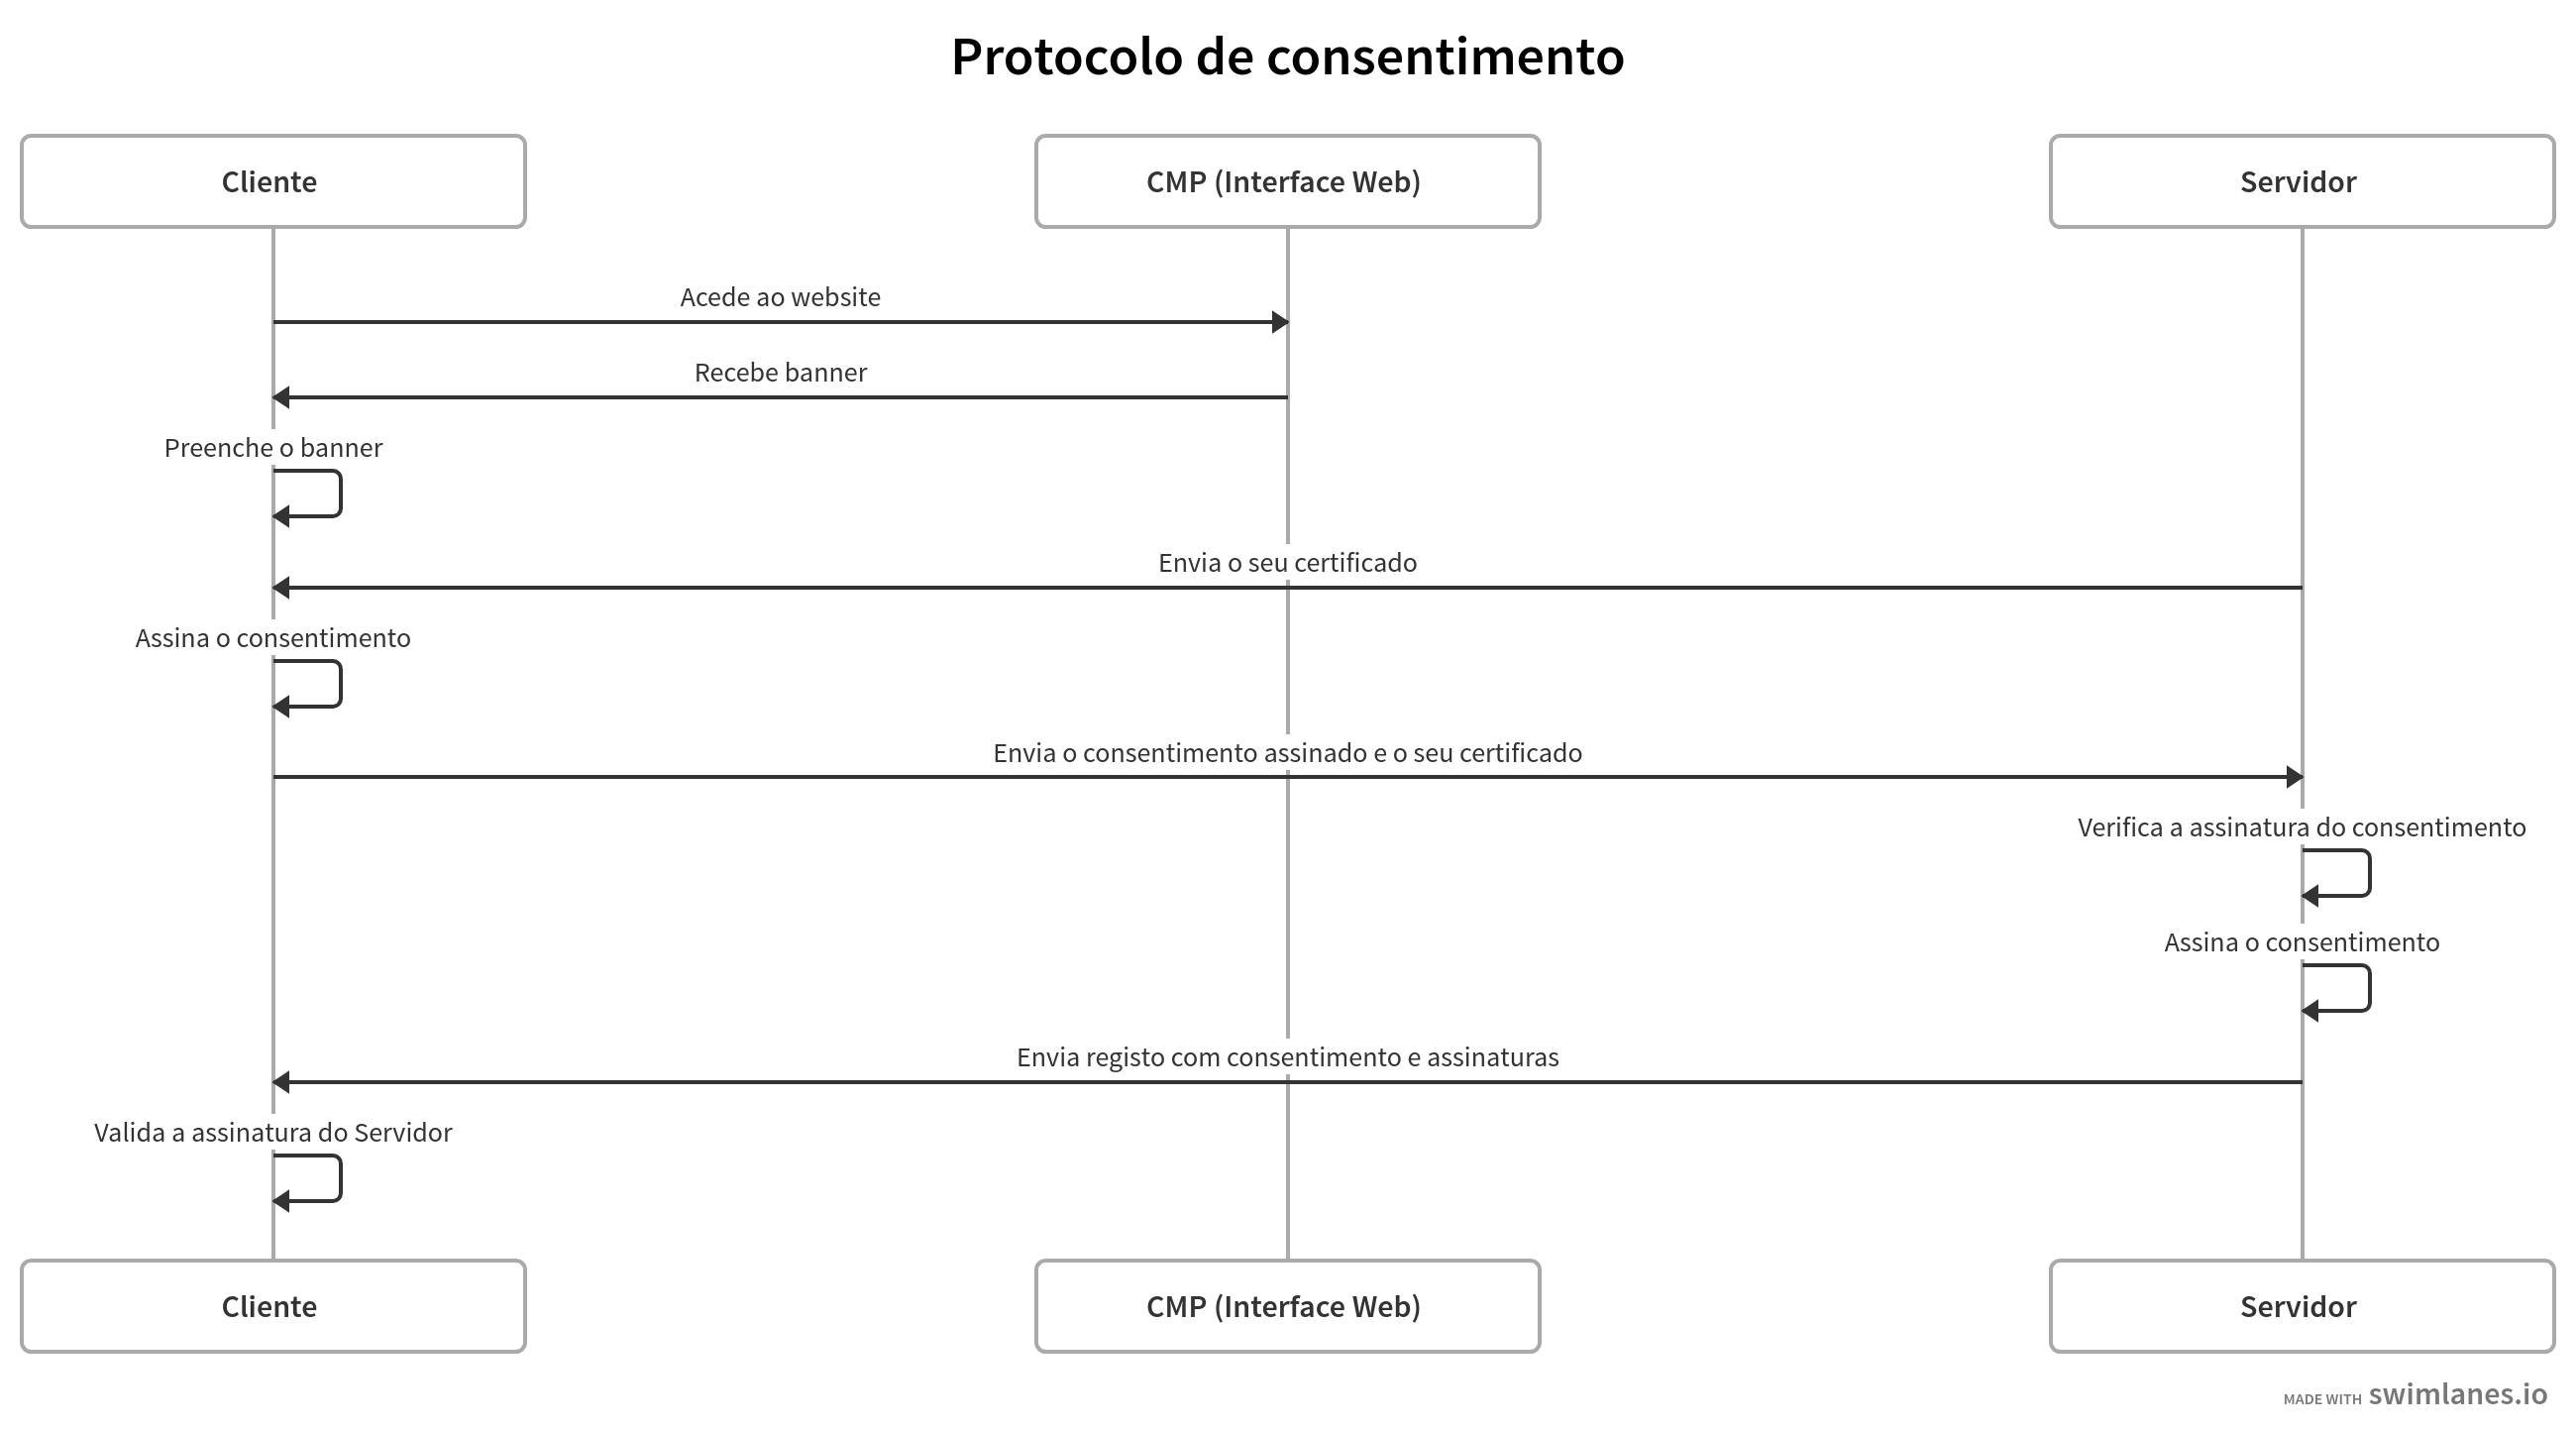
\includegraphics[width=1\textwidth]{images/swimlanes.png}
\end{center}
\caption{Diagrama do protocolo de prova de consentimento}
\end{figure}

\newpage

\section{Lógica de Funcionamento}

A estratégia proposta assenta numa abordagem de assinaturas digitais, na qual o cliente e servidor participam ativamente na criação de um registo de consentimento verificável e imutável. Esta abordagem garante quatro propriedades fundamentais: \textit{transparência}, na medida em que todos os passos podem ser verificados; \textit{descentralização}, dado que nenhuma das partes detém controlo unilateral; \textit{não-repúdio}, assegurando que os consentimentos prestados não podem ser posteriormente negados; e \textit{auditabilidade}, uma vez que o histórico completo permanece acessível tanto localmente, junto de cada entidade participante, como opcionalmente através de um serviço de terceiros responsável pela verificação ou conservação dos registos.

\section{Benefícios}

A \textit{Prova de Consentimento} proposta apresenta benefícios distintos para os diferentes intervenientes.
%Do ponto de vista do utilizador, a solução facilita aceder aos consentimentos prestados mais facilmente, assegurando transparência no processo.
Do ponto de vista do utilizador, este tem a possibilidade de verificar a integridade dos registos, garantindo que não foram alvo de manipulação, e dispõe ainda de mecanismos que lhe conferem autonomia para comprovar eventuais incumprimentos por parte do prestador de serviços.

Para as organizações, a arquitectura disponibiliza provas fiáveis de consentimentos válidos, que podem ser utilizadas em auditorias ou processos de verificação de conformidade.
Deste modo, contribui para a redução dos riscos associados ao incumprimento das regulamentações em vigor, promovendo maior confiança e segurança jurídica no tratamento de dados pessoais.

\section{Síntese do capítulo}

Neste capítulo foi apresentada a arquitectura conceptual da solução de prova de consentimento, detalhando os principais componentes, a lógica de funcionamento e os mecanismos criptográficos, como certificados digitais e assinaturas digitais. Através da Prova de Conceito, demonstrou-se a viabilidade do modelo conceptual, validando a autenticidade, integridade, não repúdio, transparência e auditabilidade dos registos de consentimento num ambiente simplificado, sem recorrer ainda a uma implementação completa.

O capítulo seguinte descreve a implementação prática desta arquitectura, materializada num protótipo funcional que integra os princípios validados na Prova de Conceito. Nesta fase, são exploradas tecnologias reais e fluxos completos, permitindo avaliar o desempenho, a interoperabilidade e a experiência de utilização, evidenciando os benefícios e limitações do sistema face às limitações identificadas no trabalho relacionado (\ref{cap:relacionado}).

\chapter{Implementação da solução}
\label{cap:implementacao}

Neste capítulo apresenta-se a prova de conceito da solução proposta, demonstrando a viabilidade da arquitetura definida no capítulo anterior, seguida da implementação da mesma. Esta permite testar os principais componentes do sistema, as tecnologias utilizadas e o fluxo de comunicação que assegura a recolha, assinatura, validação e registo do consentimento digital. Por fim, são apresentados os resultados dos testes funcionais, que permitem avaliar se a implementação cumpre os objetivos definidos para o sistema.

\section{Prova de Conceito}

O objetivo é demonstrar a viabilidade técnica e conceptual da \textit{Prova de Consentimento} apresentada no Capítulo~\ref{cap:arquitectura}, validando os princípios de autenticidade, integridade, não repúdio, transparência e auditabilidade sem recorrer a uma implementação completa.

O registo de consentimento é representado como um objeto estruturado, contendo o \textit{payload} com as decisões do utilizador, a assinatura digital do próprio utilizador (gerida através da extensão) e a assinatura digital do servidor. Esta abordagem demonstra que o sistema suporta múltiplas assinaturas sobre o mesmo conteúdo, conforme previsto na \textit{JSON Serialization} do \textit{JWS}, assegurando verificabilidade e auditabilidade mesmo num modelo simplificado.

A prova de conceito permite confirmar que é possível gerar, assinar e verificar registos de consentimento de forma independente, validando a integridade e autenticidade dos dados e assegurando o não repúdio. Além disso, evidencia que a arquitetura conceptual é flexível e pode ser posteriormente implementada num protótipo funcional com componentes reais, incluindo extensões de navegador, servidores e CMPs diferentes. Assim, esta demonstração serve como validação experimental da arquitetura, reforçando a confiança na abordagem e evidenciando os benefícios do modelo proposto.

\section{Prova de conceito e testes funcionais}

O \textit{back-end} do servidor foi desenvolvido em \textit{Node.js}, enquanto o website é constituído por uma página em \textit{HTML} simples, integrando um \textit{snippet} do \textit{script} de um \acrshort{cmp} \textit{Open-Source} (\textit{klaro.js}) para a apresentação do \textit{banner} de consentimento.
Esta escolha oferece maior flexibilidade: permite que a solução seja utilizada como base para o desenvolvimento de sistemas próprios, sem a necessidade de criar um CMP do zero. Isto reduz o esforço de implementação e facilita a integração com diferentes navegadores, serviços ou fluxos de consentimento. Para o utilizador, o benefício reside não apenas na possibilidade de verificar e auditar o funcionamento da ferramenta, mas também na garantia de que os seus consentimentos são processados de forma consistente e que a implementação pode ser adaptada para reforçar a sua privacidade e controlo sobre os dados.
Do lado do cliente, foi implementada uma extensão de navegador em JavaScript, responsável pela captura das interações do utilizador e pela execução das operações criptográficas necessárias. Embora se trate de uma extensão em JavaScript nativo, recorreu-se ao \textit{Vue.js} como \textit{framework}, em conjunto com o Vite como \textit{bundler}, de modo a permitir a integração de bibliotecas externas, nomeadamente o \texttt{node-forge} para o tratamento de chaves e certificados. Adicionalmente, o processo de criação e gestão de certificados digitais foi realizado com recurso a o \textit{OpenSSL}. O fluxo de comunicação resultante contempla as etapas de recolha, assinatura, envio, validação e registo do consentimento em ambas as entidades, assegurando a autenticidade, integridade e verificabilidade do processo.

\subsection{JWS}

No âmbito da gestão do consentimento, a organização e validação dos mesmos exigem um formato seguro, interoperável e verificável. Entre várias alternativas, optou-se por utilizar o \textit{JSON Web Signature} (\textit{JWS}), conforme definido no RFC 7515 \citep{rfc7515}.

\subsubsection{Descrição Geral}

De acordo com o RFC 7515, um \textit{JWS} representa conteúdos protegidos com assinaturas digitais ou códigos de autenticação de mensagem (MAC) \citep{NISTMAC}, usando estruturas de dados em JSON.

Existem duas formas de serialização definidas:

\begin{itemize}
  \item \textit{Compact Serialization}: uma representação mais concisa, adequada a ambientes com restrições de espaço, como cabeçalhos HTTP ou parâmetros de URL.
  \item \textit{JSON Serialization}: uma representação em JSON que permite múltiplas assinaturas ou MACs sobre o mesmo conteúdo, com maior clareza e flexibilidade.
\end{itemize}

O \textit{JWS} baseia-se em três componentes principais:

\begin{enumerate}
  \item \textit{Header}: contém metadados como o algoritmo de assinatura (por exemplo, \texttt{PS256} \citep{Auth0SigningAlgorithms}), o tipo de objeto (por exemplo, \texttt{JWT}), e possivelmente outros parâmetros relevantes.
  \item \textit{Payload}: o conteúdo a assinar que é codificado em Base64URL.
  \item \textit{Signature}: o resultado da assinatura digital aplicada ao \textit{header} e \textit{payload}, garantindo integridade e autenticidade.
\end{enumerate}

\subsubsection{Aplicação ao Caso de Consentimento}

No sistema implementado, o consentimento do utilizador é representado através de um \textit{JWS}, com estas características específicas:

\begin{itemize}
  \item O \textit{payload} inclui informação relevante sobre o consentimento (por exemplo, serviços aceites/rejeitados).
  \item O \textit{header} utiliza o algoritmo \texttt{PS256}, que combina RSASSA-PSS com SHA-256, tendo sido escolhido devido às suas vantagens de segurança face ao RS256. O PS256 utiliza o esquema de preenchimento probabilístico (PSS), gerando assinaturas diferentes para o mesmo \textit{header} e \textit{payload}, o que aumenta a resistência contra ataques a assinaturas determinísticas e fornece maior robustez criptográfica \citep{ScottBrady2020}.
  \item São produzidas, pelo menos, duas assinaturas:
    \begin{itemize}
      \item Uma assinatura gerada pelo cliente (extensão do navegador), garantindo que foi o utilizador quem autorizou o consentimento.
      \item Outra assinatura adicional do servidor, garantindo que o servidor valida e “assina” o consentimento final, reforçando a confiabilidade e verificabilidade.
    \end{itemize}
\item A presença de múltiplas assinaturas segue o modelo da \textit{JSON Serialization} do \textit{JWS}, que suporta várias assinaturas sobre o mesmo \textit{payload}.
\end{itemize}

\subsubsection{Vantagens neste contexto}

Neste contexto, a utilização do \textit{JWS} oferece várias vantagens. Em primeiro lugar, garante a integridade e autenticidade do consentimento, uma vez que qualquer modificação no \textit{payload} ou nas assinaturas invalida o \textit{JWS}, protegendo contra manipulação. 
Em segundo lugar, assegura o não repúdio, uma vez que as assinaturas do cliente e do servidor permitem verificar se o consentimento foi efetivamente fornecido pelo utilizador e validado pelo servidor.
Além disso, tanto o cliente como o servidor conseguem verificar de forma independente a autenticidade do consentimento, reforçando a confiança no processo.
Por fim, o \textit{JWS} segue padrões abertos e é interoperável, o que facilita a integração com outras ferramentas e sistemas, permitindo que os registos de consentimento sejam utilizados de forma consistente em diferentes contextos e aplicações.

\begin{itemize}
  \item Integridade e Autenticidade: Qualquer modificação no \textit{payload} ou nas assinaturas invalida o \textit{JWS}, protegendo contra manipulação.
  \item Não repúdio: A assinatura do servidor impede que este negue ter dado o consentimento, sendo uma evidência legalmente relevante.
  \item Verificabilidade por ambas as partes: Cliente e servidor conseguem validar, de forma independente, que o consentimento é autêntico e válido.
  \item Compatível com padrões e interoperável: Facilita futuras integrações com outras ferramentas.
\end{itemize}


\subsection{Servidor e Website}

Para capturar a interação do \acrshort{ds}, é disponibilizado um website estático em HTML, no qual se integra o \textit{script} do \textit{klaro.js}, seguindo a prática comum na implementação de \acrshort{cmp}s.
É possível definir quais são os serviços usados em um ficheiro chamado \texttt{config.js} que deve estar estruturado como o exemplo disponibilizado pelo \cite{gitklaro}. Neste caso, como não têm relevância quais os serviços a ser utilizados, foram mantidos os valores por omissão.

% adicionar ao avaliacoes?
Pode-se ver um exemplo de serviço configurado (Listagem~\ref{lst:klaro-service-example}):


\begin{lstlisting}[language=Javascript, caption={Exemplo de serviço configurado no \textit{klaro.js}}, label={lst:klaro-service-example}]
// This is a list of third-party services that Klaro will manage for you.
services: [
	{
		name: 'twitter',
		default: false,
		contextualConsentOnly: true,
		purposes: ['marketing'],
	},
\end{lstlisting}

Este ficheiro é depois chamado no referido \textit{script} anteriormente \textit{klaro.js}, que se trata de uma complilação de tudo que compõe o \acrshort{cmp} \textit{klaro.js}. Aqui, é possível chamar o \textit{script} através de um \textit{endpoint} exposto pelo próprio desenvolvedor da ferramenta, ou então importar para o projeto. Nesta solução, foi escolhido o segundo método para a utilização da configuração.
Sendo assim só foi necessário chamar estes dois \textit{scripts} para implementar o serviço (ver Listagem~\ref{lst:klaro-integration}).

\begin{lstlisting}[language=HTML, caption={Integração do \textit{klaro.js} com a configuração local}, label={lst:klaro-integration}]
<!DOCTYPE html>
<html lang="en">
<head>
    <meta charset="UTF-8">
    <title>Consent Management POC</title>

    <script defer type="text/javascript" src="config.js"></script>
    <script defer type="text/javascript" src="klaro.js"></script>
</head>
...
\end{lstlisting}

Assim, tem-se as ferramentas necessárias para ter um ponto de interação com o \acrshort{ds}.

Toda a lógica de troca de consentimento e de certificados é suportada por um servidor \textit{back-end}, desenvolvido em NodeJS, que expõe dois \textit{endpoints} principais para comunicação com o cliente.

O primeiro \textit{endpoint}, acessível através de um pedido \texttt{GET} em \texttt{/api/server\_certificate}, devolve o certificado do servidor. Este certificado é utilizado pelo cliente para validar as comunicações e garantir a autenticidade das assinaturas digitais. Em caso de sucesso, o certificado é devolvido em formato \texttt{JSON}, caso contrário, o servidor responde com o respetivo erro.

O segundo \textit{endpoint}, acessível através de um pedido \texttt{POST} em \texttt{/api/consent}, recebe do cliente um consentimento assinado no formato \textit{JWS}. O corpo da requisição inclui a chave pública do cliente, o consentimento propriamente dito e a assinatura associada. O servidor procede então a várias operações:

\begin{enumerate}
    \item Verificação da assinatura do cliente: utilizando a chave pública fornecida através do certificado, confirma-se que o consentimento foi efetivamente assinado pelo cliente, assegurando a integridade e autenticidade da informação recebida.
    \item Criação de um objeto \textit{JWS} assinado pelo servidor e cliente: após validação, o consentimento é encapsulado na estrutura \textit{JWS}, assinado com a chave privada do servidor, de modo a gerar evidência verificável para ambas as partes.
    \item Resposta ao cliente: é devolvido ao cliente um objeto em formato \texttt{JSON}, contendo o \textit{JWS} assinado pelo cliente e servidor e uma mensagem de confirmação. Em caso de falha, é emitida uma resposta de erro.
\end{enumerate}

A implementação completa dos \textit{endpoints} e da lógica de verificação e assinatura pode ser consultada no Apêndice~\ref{apendice:server-endpoints}.

Deste modo, o servidor é responsável por validar as mensagens recebidas e por emitir, como resposta, um \textit{JWS} assinado com a sua chave privada. Esse \textit{JWS} não constitui, por si só, a conclusão do processo: é posteriormente validado pelo cliente com recurso ao certificado público obtido em \texttt{/api/server\_certificate}, confirmando a autenticidade da assinatura do servidor e a integridade/consistência do \textit{payload} antes de proceder ao registo local do consentimento.

\subsection{Extensão no Cliente}
Do lado do cliente desenvolveu-se uma extensão para o navegador \textit{Firefox}, responsável pela gestão da troca de consentimentos. Esta foi implementada em JavaScript \citep{MozillaBrowserExtensions}. O manifest é um ficheiro de configuração obrigatório em qualquer extensão de navegador, que define informações essenciais sobre a extensão, como nome, versão, permissões, \textit{scripts} a executar e outros recursos necessários para o seu funcionamento. O \texttt{manifest v3} foi uma atualização do formato usado pelas extensões, focada sobretudo em reforçar a segurança e privacidade, limitando certas funcionalidades usadas por \textit{ad blockers} e \textit{scripts} de terceiros. No entanto, para a extensão desenvolvida a migração do v2 para o v3 não trouxe diferenças práticas significativas, uma vez que o seu funcionamento não depende das funcionalidades que foram restringidas nesta atualização.

\subsubsection{Module Bundlers}

Durante o desenvolvimento da extensão em JavaScript, foi necessário recorrer a um \textit{module bundler} para gerir as bibliotecas externas e garantir compatibilidade entre navegadores. Para tal, utilizou-se o Vite, ferramenta padrão do \textit{Vue.js}, que simplifica a integração das dependências e a preparação do código para testes e distribuição. O Vite permitiu organizar o código e as dependências de forma eficiente, facilitando o desenvolvimento e a disponibilização da extensão.

\subsection{Gestão de Certificados}
Para a criação dos certificados, foi usada a ferramenta do OpenSSL para testes locais. Para obter estes mesmos certificados por parte do servidor e cliente, procedemos à criação de uma rootCA. Sendo assim, neste caso, ambas utilizam a mesma root CA. Os certificados utilizados na solução são do tipo \textit{X.509 v3}. Com isto, é necessário também que cada uma das entidades tenha a sua chave privada.

Detalhes sobre a criação dos certificados e das chaves podem ser encontrados no Apêndice~\ref{ap:certificados}.

No entanto, a extensão necessita ainda de aceder ao certificado e à chave privada do cliente (\texttt{client.crt} e \texttt{client.key}). Estes são armazenados no \textit{local storage} do navegador e carregados pela própria extensão, como é visível na Listagem~\ref{lst:client-cert-load}.

\begin{lstlisting}[language=Javascript, caption={Carregamento do certificado e da chave privada do cliente a partir do \textit{local storage}}, label={lst:client-cert-load}]
...
certPEM = localStorage.getItem("cert");
certPEM = this.formatPem(certPEM, "CERTIFICATE");

privKey = localStorage.getItem("privKey");
privKey = this.formatPem(privKey, "PRIVATE KEY");
...
\end{lstlisting}

A integração com o módulo \texttt{node-forge} foi utilizada para o tratamento e gestão de chaves criptográficas e certificados digitais, suportando as operações de assinatura e verificação do sistema. Mas como em extensões de navegador apenas é permitido código JavaScript nativo, foi necessário proceder à sua compilação e empacotamento. Para tal, recorreu-se a um \textit{bundler}, tendo sido escolhida a \textit{framework} \textit{VueJS} \citep{VueJS}.

Quer do lado do servidor, quer do lado do cliente, a gestão de chaves e certificados é simplificada através do recurso ao \texttt{node-forge}. O servidor realiza o carregamento das chaves RSA e do certificado diretamente a partir do sistema de ficheiros, extraindo os elementos necessários para validação e assinatura dos consentimentos.

O seguinte excerto de código (Listagem~\ref{lst:server-rsa-key-load}) demonstra a lógica implementada:

\begin{lstlisting}[language=Javascript, caption={Carregamento das chaves RSA do servidor e do certificado associado}, label={lst:server-rsa-key-load}]
loadRSASigningKeys() {
	const certPem = fs.readFileSync('server.crt', 'utf8');
	const cert = forge.pki.certificateFromPem(certPem);
	const publicKey = forge.pki.publicKeyToPem(cert.publicKey);

	const privateKey = fs.readFileSync('server.key', 'utf8');

	this.serverKeys.rsaPrivateSigningKey = privateKey;
	this.serverKeys.rsaPublicSigningKey = publicKey;
	this.serverCert = certPem;
}
\end{lstlisting}

Neste processo:
\begin{itemize}
    \item O certificado do servidor é lido e decodificado em formato PEM, permitindo extrair a chave pública para validação das assinaturas.
    \item A chave privada é carregada diretamente do ficheiro correspondente, sendo utilizada para assinar os \textit{JWS} recebidos do cliente.
    \item O \texttt{node-forge} facilita a manipulação de certificados e a conversão entre formatos PEM e objetos manipuláveis em JavaScript.
\end{itemize}

\subsection{Fluxo de Consentimento}

O processo inicia-se quando o utilizador interage com o \textit{banner} de consentimento (aceitação ou rejeição), disponibilizado pelo \textit{Klaro.js} (Figura~\ref{fig:klarojs-banner}).

\begin{figure}[h]
    \centering
	
\includegraphics[width=0.8\textwidth]{images/klaro_banner.png}
	\caption{Banner padrão do \textit{klaro.js}.}
\label{fig:klarojs-banner}
\end{figure}

A extensão do navegador captura este evento através de um \textit{listener}, que desencadeia a função principal \texttt{processConsent}. Este processo caracteriza-se pelas seguintes etapas:
\begin{enumerate}
    \item Obtenção do certificado digital do servidor, essencial para validar a autenticidade das mensagens recebidas.
    \item Carregamento das chaves do cliente (\texttt{client.key} e \texttt{client.crt}) do \textit{local storage}.
    \item Assinatura digital do consentimento pelo cliente, criando uma evidência verificável.
    \item Envio do consentimento assinado ao servidor.
    \item Validação do consentimento no servidor, incluindo a verificação da assinatura do cliente.
    \item Criação de um \textit{JWS} assinado pelo servidor e envio de resposta ao cliente.
    \item Validação final do \textit{JWS} pelo cliente, assegurando a integridade e autenticidade do \textit{payload} antes de registar localmente o consentimento.
\end{enumerate}

Este fluxo garante que todas as interações são auditáveis, permitindo rastreabilidade e conformidade com requisitos legais de proteção de dados.

Para maior detalhe sobre a implementação prática deste fluxo, incluindo a captura do evento de consentimento, assinatura digital, envio ao servidor e verificação do \textit{JWS}, pode ser consultado o Apêndice~\ref{apendice:process-consent}, onde a função \texttt{processConsent} é apresentada na íntegra.

O fluxo descrito pode ser visualizado no diagrama da Figura~\ref{fig:swimlane-solution}.

\begin{figure}[h]
\begin{center}
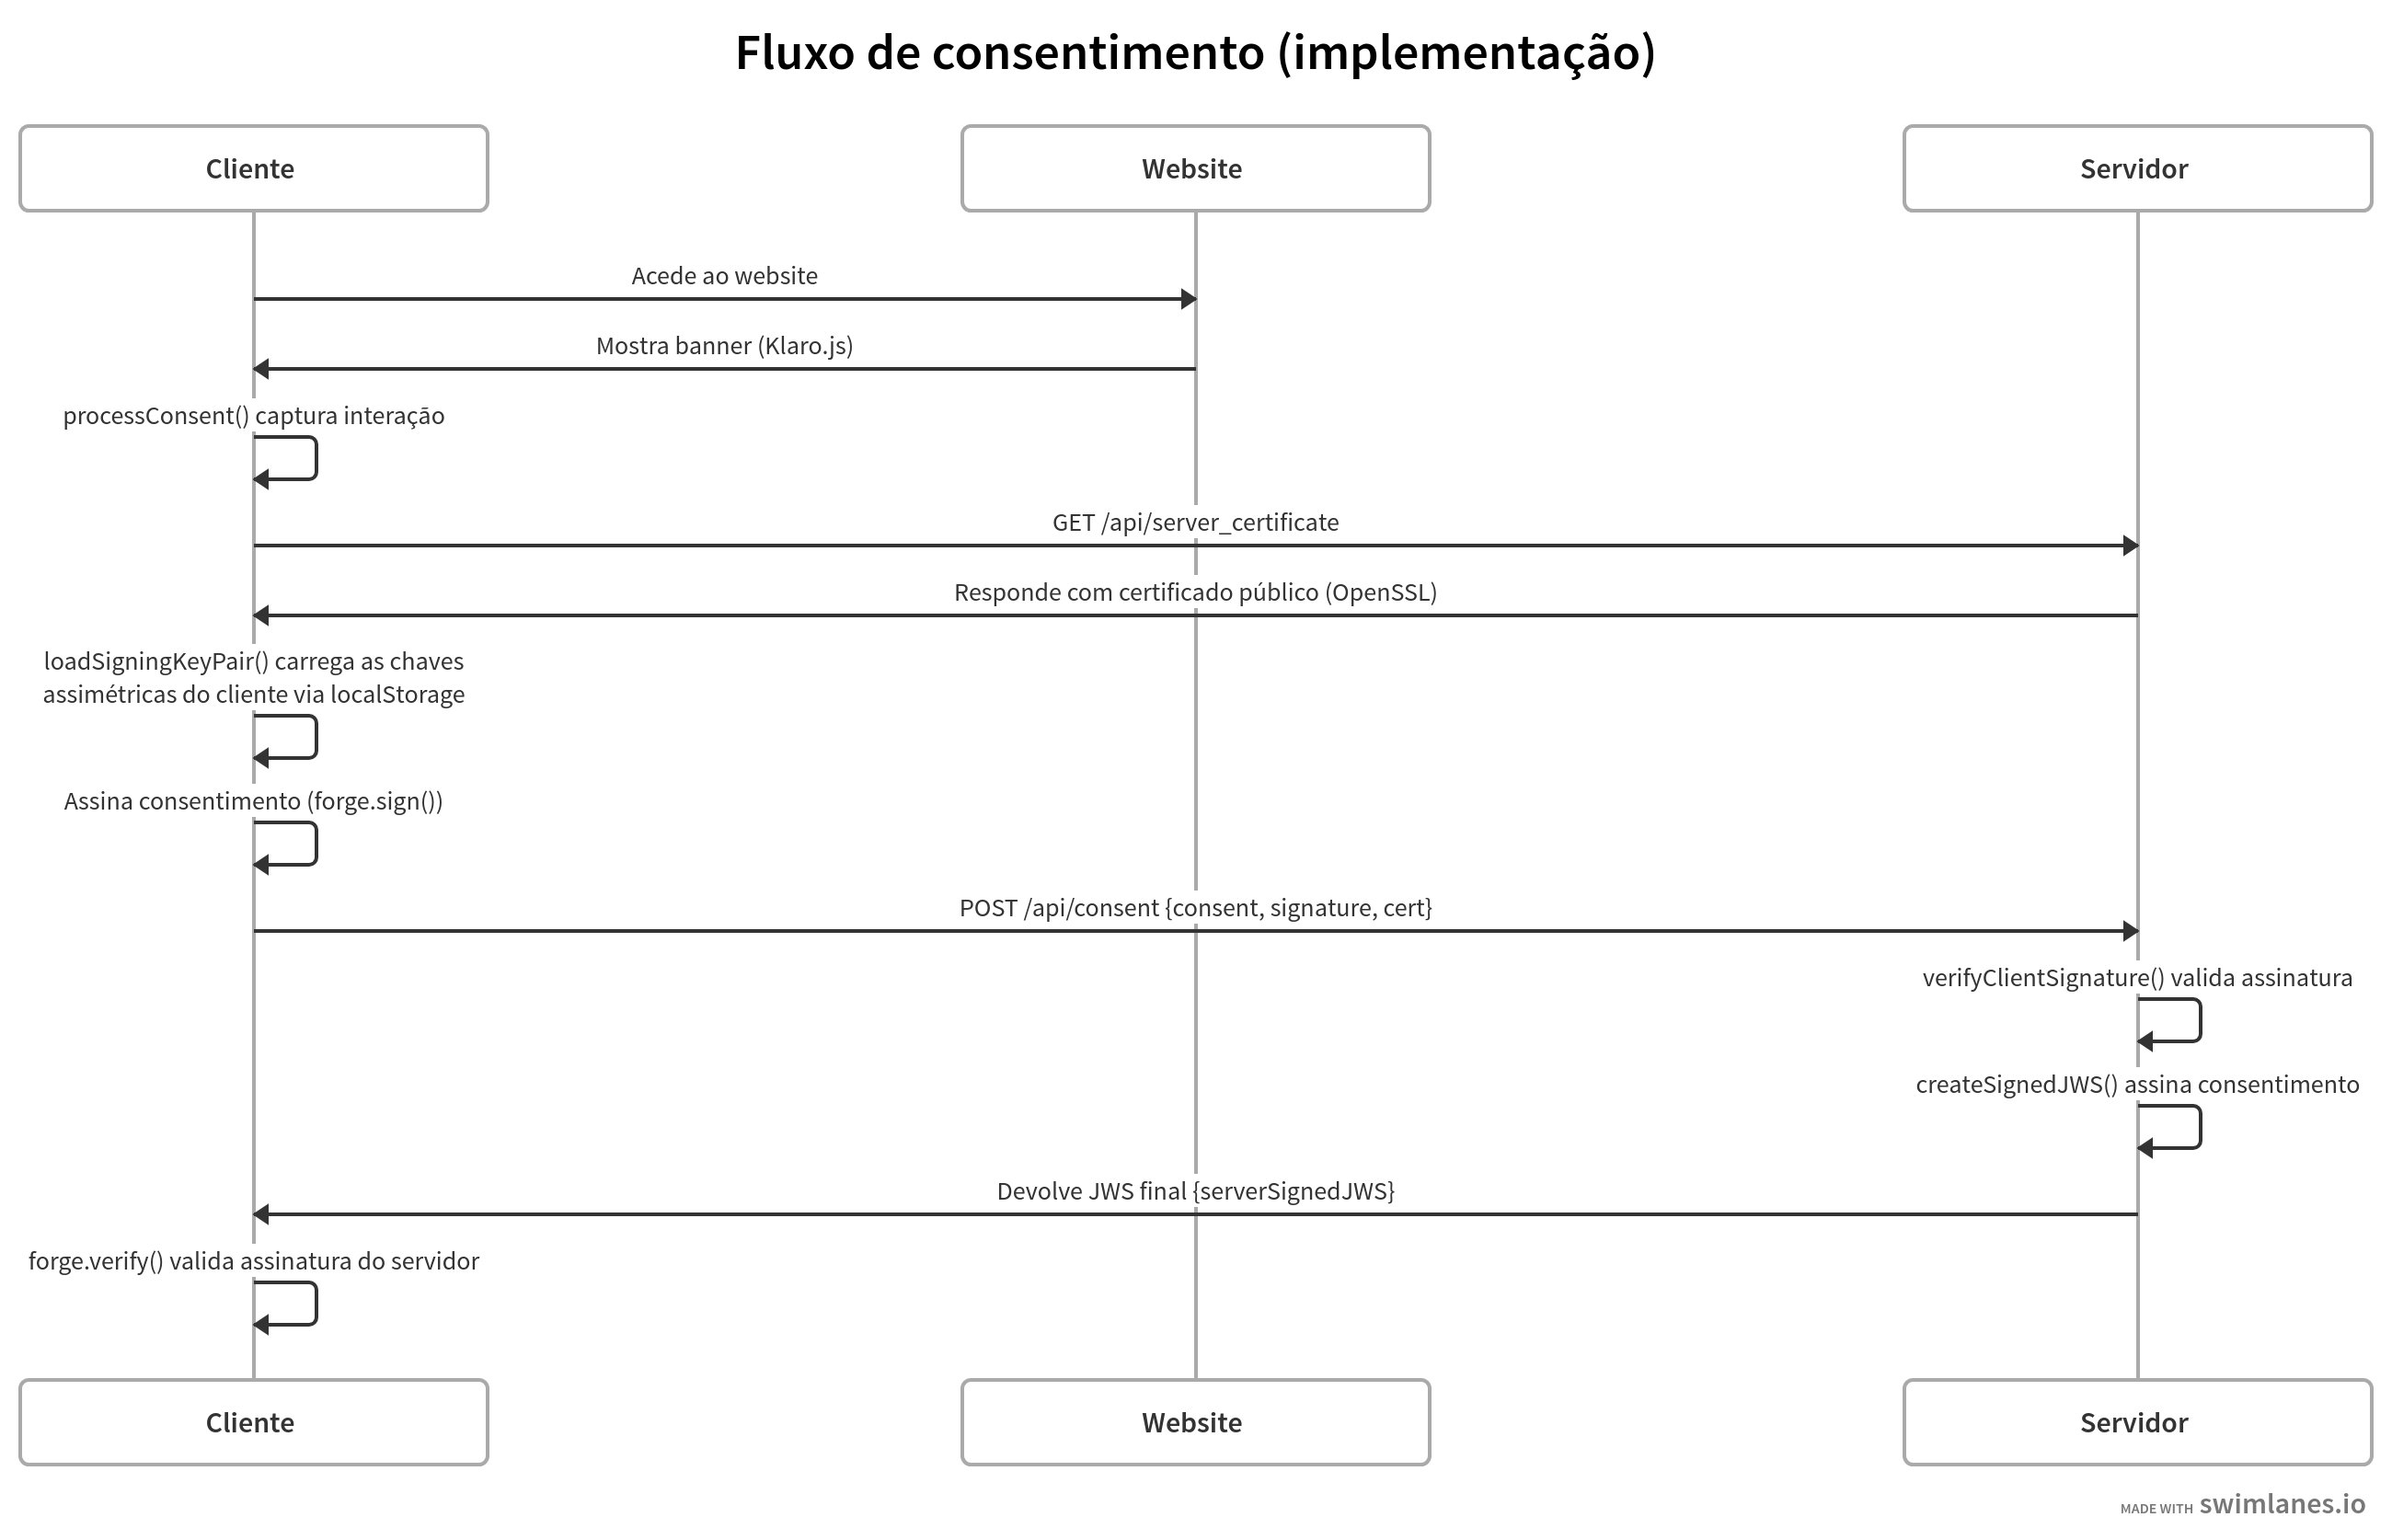
\includegraphics[width=1\textwidth]{images/swimlanes_solution.png}
\end{center}
\caption{Diagrama do protocolo.}
\label{fig:swimlane-solution}
\end{figure}

\newpage

\subsection{Registo do consentimento}

O registo do consentimento, juntamente com as respetivas assinaturas, constitui o resultado final do fluxo implementado. Trata-se de um registo digital que comprova a aceitação ou rejeição, pelo utilizador, de determinados serviços ou finalidades. Este registo é implementado sob a forma de um \textit{JSON Web Signature} (\textit{JWS}), que encapsula o \textit{payload} com os detalhes do consentimento do utilizador, a assinatura digital do cliente — garantindo que foi efetivamente o utilizador a autorizar — e a assinatura digital do servidor, que confirma a validação e integridade do consentimento.

O \textit{JWS} é mantido por ambas as entidades, cliente e servidor, permitindo consultas futuras, auditoria e eventual revogação do consentimento. Este mecanismo assegura a \textit{autenticidade}, uma vez que a assinatura do cliente comprova que o consentimento foi emitido pela pessoa correta; a \textit{integridade}, já que qualquer alteração no \textit{payload} invalida as assinaturas e impede a manipulação; e o \textit{não repúdio}, pois o cliente não pode negar a sua decisão devido à assinatura digital inequívoca, nem o servidor pode negar que conhece a decisão do utilizador.

Podemos consultar no apêndice \ref{apendice:jws-client} a implementação do \textit{JWS} do lado do cliente.

O \textit{JWS} resultante contém dois elementos principais:

\begin{itemize}
    \item \textit{Payload}: o \textit{payload} codificado em \textit{base64} com os dados do consentimento do utilizador.
    \item \textit{Signatures}: um array com uma ou mais assinaturas digitais. Neste caso, inclui a assinatura do cliente e a assinatura do servidor.
\end{itemize}

Um exemplo de \textit{JWS} gerado é o seguinte:

\begin{lstlisting}
{
  "payload": "eyJjb25zZW50cyI6eyJ0d2l0dGVyIjpmYWxzZSw ...",
  "signatures": [
    {
      "header": {"typ": "JWT", "alg": "PS256"},
      "signature": "b1Xn5AaxYZWZNfHoeL-SWTAySbT8yFWjJiPTK_rlIoPwTdukp9wpn..."
    },
    {
      "header": {"typ": "JWT", "alg": "PS256"},
      "signature": "BPVz73atRIFhzRx6YVsHWOkEX6Rb-hL0XoahOc2uxX9EPDs5RSVvYuNzpoX_Vv..."
    }
  ]
}
\end{lstlisting}

Esta estrutura assegura que tanto o cliente como o servidor possuem uma prova verificável do consentimento, permitindo auditoria, revogação ou consulta futura. Deste modo, o mecanismo implementado cumpre os objetivos definidos na criação desta prova de conceito, pois fornece uma forma de registar e gerir consentimentos de forma transparente e técnica, garantindo a criação de registos verificáveis, imutáveis e não repudiáveis.

A solução permite não só a recolha e gestão dos consentimentos dos utilizadores, mas também possibilita auditar os consentimentos em caso de não cumprimento, promovendo a transparência e fornecendo evidência técnica irrefutável de que as decisões dos utilizadores foram, ou não foram, respeitadas no tratamento dos dados. Embora não garanta a conformidade integral dos prestadores de serviços com regulamentos como o \acrshort{rgpd}, o sistema permite aos utilizadores demonstrar a não-conformidade em caso de violação das suas escolhas de privacidade, cumprindo assim os objetivos principais do projeto. Os testes funcionais e de desempenho descritos no Capítulo~\ref{cap:avaliacao} confirmam a viabilidade do modelo, validando o fluxo de consentimento, a criação e verificação de \textit{JWS} e a robustez das assinaturas digitais.

\section{Síntese do capítulo}

Neste capítulo foram apresentadas duas fases complementares da implementação da solução proposta. A prova de conceito permitiu validar a arquitetura conceptual, demonstrando a viabilidade técnica dos princípios de integridade, autenticidade, não repúdio, transparência e auditabilidade num modelo simplificado. Seguiu-se o desenvolvimento da prova de conceito, integrando cliente, servidor e interface web, com a utilização de certificados digitais, assinaturas e o formato \textit{JWS} para criar registos de consentimento auditáveis e verificáveis. Foram realizados testes funcionais e de desempenho, descritos no Capítulo~\ref{cap:avaliacao}, que confirmaram o correto funcionamento do fluxo de consentimento e a robustez das assinaturas digitais.  

No capítulo seguinte é apresentada a avaliação da implementação, abordando tanto os aspetos funcionais como de desempenho. Serão analisados os testes realizados e os resultados obtidos, de forma a demonstrar a fiabilidade, robustez e eficiência da arquitetura desenvolvida, evidenciando o cumprimento dos objetivos definidos neste trabalho.

\chapter{Avaliação}
\label{cap:avaliacao}

Capitulo avaliação. Printscreens da solução, mostrar o conteudo de algumas coisas. tentar avaliar quanto tempo demora a cifragem, se aumentar o conteudo do payload muda.

\chapter{Conclusões e trabalho futuro}
\label{cap:conclusoes}

\section{Conclusões}

O principal objetivo definido para este trabalho consistia em conceber e prototipar um sistema de gestão de consentimento que, para além de recolher as escolhas do utilizador, permitisse também auditar o processo de forma transparente e verificável caso fosse necessário. Para tal, partiu-se da análise crítica das limitações das \acrshort{cmp}s tradicionais, em particular a falta de transparência e de mecanismos de auditoria, e delineou-se uma solução que permitisse acrescentar estas garantias independentemente da plataforma utilizada. A proposta sugere funcionalidades que podem ser aplicados em qualquer \acrshort{cmp} existente, potenciando a transparência e a verificabilidade do processo de gestão de consentimento.

Este objetivo foi alcançado através da definição de uma arquitetura genérica baseada em três entidades principais (utilizador, extensão no navegador e servidor), capaz de registar consentimentos com recurso a assinaturas digitais e certificados. A implementação prática validou a viabilidade deste modelo, recorrendo a tecnologias como \textit{Node.js} no servidor, \textit{klaro.js} para o \textit{banner} de consentimento e uma extensão de navegador em JavaScript, suportada por bibliotecas de criptografia. O processo resultou num fluxo completo de recolha, assinatura, validação e registo de consentimentos em formato \textit{JWS}, garantindo autenticidade, integridade, não repúdio e auditabilidade.

Desta forma, pode afirmar-se que os objetivos delineados foram cumpridos. A solução concebida não só demonstra ser possível conjugar simplicidade de utilização com garantias de segurança e confiança, como também responde diretamente ao principal problema identificado: a ausência de mecanismos que permitam ao utilizador salvaguardar-se em caso de não conformidade. Com o registo duplamente assinado em formato \textit{JWS}, o utilizador dispõe de uma prova verificável do consentimento que efetivamente forneceu, podendo assim contestar eventuais falhas do lado do prestador de serviços. Esta arquitetura constitui o contributo mais relevante desta dissertação, ao assegurar que tanto utilizador como organização partilham um histórico comum, transparente e verificável.

%Apesar de não ter sido integrada nesta fase, a extensão do workflow com blockchain foi também considerada, tendo sido apresentado um esboço de como poderia reforçar a imutabilidade e a confiança nos registos de consentimento. Este ponto abre caminho para trabalho futuro, assim como a avaliação em cenários mais próximos de ambientes de produção, permitindo aferir o desempenho, escalabilidade e aplicabilidade em contextos organizacionais de maior dimensão.

\section{Trabalho futuro}

Embora a solução apresentada tenha demonstrado a viabilidade de integrar mecanismos de auditoria e verificação de consentimentos em plataformas existentes, permanecem diversas oportunidades para evolução e aprofundamento do trabalho. Esta secção discute possíveis direções para trabalhos futuros, destacando melhorias técnicas e expansão de funcionalidades que possam aumentar a transparência, a confiabilidade e a escalabilidade do sistema. O objetivo é fornecer uma perspetiva sobre como a investigação presente pode ser prolongada, contribuindo para soluções mais robustas e abrangentes no domínio da gestão de consentimento de dados.

\subsection{Complementação do fluxo com \textit{blockchain} e contratos inteligentes}

A prova de conceito desenvolvida assegura a autenticidade, integridade e verificabilidade dos consentimentos através de assinaturas digitais e certificados. No entanto, uma possível extensão futura seria a integração com um \textit{ledger} público.

A utilização desta tecnologia permitiria reforçar a imutabilidade dos registos, uma vez que o consentimento poderia ser armazenado de forma distribuída numa rede pública, resistente a manipulações. Neste cenário, após o consentimento ser validado e assinado por ambas as partes, o servidor poderia proceder ao registo do identificador único associado ao consentimento (ID) numa \textit{blockchain} pública, como a \textit{Ethereum}.

Com este mecanismo, seria possível garantir que qualquer entidade interessada, incluindo o próprio utilizador, pudesse verificar, de forma independente, a existência e consistência dos consentimentos registados. O registo em \textit{blockchain} funcionaria, assim, como uma prova adicional de confiança, complementando as garantias já oferecidas pelo sistema atual.  

Importa salientar que, na integração com \textit{blockchain}, apenas identificadores ou \textit{hashes} dos consentimentos seriam registados, enquanto os conteúdos permaneceriam cifrados. Caso os dados completos fossem colocados diretamente na \textit{blockchain} sem cuidado, existiria o risco de rastreabilidade das ações dos utilizadores, permitindo a monitorização das suas escolhas de consentimento e atividade online. Ao manter os conteúdos cifrados, esta abordagem assegura que a imutabilidade e auditabilidade do registo não comprometem a privacidade nem a confidencialidade dos utilizadores.

Além disso, esta abordagem abriria caminho para auditorias independentes e mecanismos automatizados de verificação, assegurando que os consentimentos mantêm-se inalterados ao longo do tempo e promovendo uma maior transparência na gestão de dados pessoais.

A exploração desta integração com \textit{blockchain} e contratos inteligentes constitui, portanto, um rumo relevante para trabalho futuro, potenciando a robustez e a confiança da solução aqui apresentada.

\subsection{Integração com keychain do sistema do cliente}

Outra direção futura consiste em explorar a integração da extensão com a importação da \textit{keychain} do sistema operativo do utilizador. Esta integração permitiria gerir de forma mais segura as chaves privadas utilizadas na assinatura dos consentimentos, reduzindo o risco de exposição ou uso indevido. Além disso, garantiria maior comodidade para o utilizador, que não precisaria de gerir manualmente chaves criptográficas nem depender de soluções externas para armazenar credenciais sensíveis.

\subsection{Disponibilização da solução como projeto Open-source}

Um objetivo adicional é tornar a solução disponível como projeto \textit{Open-source}. Esta abordagem facilitaria auditorias independentes, fomentaria a confiança por parte dos utilizadores e permitiria que a comunidade contribuísse para melhorias, correções de segurança e evolução da plataforma. A abertura do código reforçaria ainda a transparência e a auditabilidade do sistema, promovendo uma adoção mais ampla em contextos académicos, corporativos e de investigação.

%\chapter{Planeamento}

\begin{table}[H]
\centering
\renewcommand{\arraystretch}{1.3} % Ajusta a altura das linhas
\setlength{\tabcolsep}{4pt} % Ajusta o espaçamento entre as colunas
\resizebox{\textwidth}{!}{%
\begin{tabular}{| c | c | c | c | c | c | c | c | c | c | c | c | c |}
\hline
\textbf{Tarefa} & \textbf{Out} & \textbf{Nov} & \textbf{Dez} & \textbf{Jan} & \textbf{Fev} & \textbf{Mar} & \textbf{Abr} & \textbf{Mai} & \textbf{Jun} & \textbf{Jul} & \textbf{Ag} & \textbf{Set} \\
\hline
\textit{Background} e \acrshort{eda} & $\bullet$ & $\bullet$ & $\bullet$ & & & & & & & & & \\
\hline
Estudo de abordagens & & $\bullet$ & $\bullet$ & $\bullet$ & & & & & & & & \\
\hline
Análise de Fluxos de Dados & & & & $\bullet$ & $\bullet$ & $\bullet$ & & & & & & \\
\hline
Desenho da Solução & & & & & & $\bullet$ & $\bullet$ & & & & & \\
\hline
Desenvolvimento da Solução & & & & & & & $\bullet$ & $\bullet$ & $\bullet$ & $\bullet$ & & \\
\hline
Otimização do sistema & & & & & & & & & & $\bullet$ & $\bullet$ & \\
\hline
Redação e Revisão da Dissertação & & & & & & & & & & & $\bullet$ & $\bullet$ \\
\hline
\end{tabular}%
}
\caption{Plano de atividades.}
\label{tab:plano-atividades}
\end{table}


\begin{enumerate} 
    \item \textbf{Background e \acrlong{eda} (Outubro - Dezembro 2024)} \\
    \textbf{Objetivo}: Realizar uma pesquisa aprofundada sobre as tecnologias e metodologias existentes no domínio de \acrfull{cmp}. A pesquisa centrada na análise das soluções atuais, como Osano, Cookiebot, Tarteaucitron.js e Google Consent Mode. Também será explorado o impacto das regulamentações como o \acrshort{rgpd} na gestão de consentimento.
    
    \textbf{Tarefas}:
    \begin{itemize}
        \item Estudo e documentação das práticas atuais de gestão de consentimento.
        \item Análise de regulamentações como o \acrshort{rgpd} e sua aplicação nas \acrshort{cmp}'s.
    \end{itemize}

    \item \textbf{Estudo de abordagens (Novembro 2024 - Janeiro 2025)} \\
    \textbf{Objetivo}: Examinar abordagens e técnicas existentes para a gestão de consentimento e auditoria de dados, considerando alternativas tecnológicas que possam ser incorporadas na solução proposta.
    
    \textbf{Tarefas}:
    \begin{itemize}
        \item Análise de técnicas de recolha e armazenamento de consentimento.
        \item Investigação sobre o uso do \textbf{CookieChimp}, incluindo testes e análise da sua \acrshort{api}.
        \item Leitura de artigos sobre \textbf{\textit{blockchain}} e \textbf{smart contracts} para possível uso na gestão de consentimento e auditoria.
    \end{itemize}

    \item \textbf{Análise de Fluxos de Dados (Janeiro - Março 2025)} \\
    \textbf{Objetivo}: Analisar os fluxos de dados típicos de um cliente até à plataforma de gestão de consentimento e avaliar as tecnologias disponíveis para garantir a auditabilidade desses fluxos, com especial ênfase no uso de \textit{blockchain} e contratos inteligentes.
    
    \textbf{Tarefas}:
    \begin{itemize}
        \item Estudo de casos práticos de fluxos de dados em plataformas \acrshort{cmp}.
        \item Seleção das tecnologias mais adequadas para garantir a transparência e a rastreabilidade desses fluxos.
        \item Análise dos desafios da auditoria de dados com \textit{blockchain} e a viabilidade do uso de smart contracts.
    \end{itemize}

    \item \textbf{Desenho da Solução (Fevereiro - Março 2025)} \\
    \textbf{Objetivo}: Desenvolver o design da solução auditável de gestão de consentimento. A solução deverá integrar a recolha de consentimento e mecanismos de auditoria, com a possibilidade de utilização de tecnologias como \textit{blockchain} para garantir a transparência.
    
    \textbf{Tarefas}:
    \begin{itemize}
        \item Desenho do modelo de dados e arquitetura do sistema.
        \item Definição das principais funcionalidades da plataforma.
    \end{itemize}

    \item \textbf{Desenvolvimento do Protótipo (Março - Maio 2025)} \\
    \textbf{Objetivo}: Desenvolver um protótipo funcional do sistema, com foco na recolha, armazenamento e auditoria do consentimento de dados.
     
    \textbf{Tarefas}:
    \begin{itemize}
        \item Implementação inicial do protótipo, com funcionalidades básicas de recolha de consentimento.
        \item Armazenamento de consentimento através da \textit{blockchain}.
        \item Integração com contratos inteligentes.
        \item Testes preliminares de usabilidade.
    \end{itemize}

    \item \textbf{Otimização do Sistema (Junho - Julho 2025)} \\
    \textbf{Objetivo}: Melhorar a usabilidade e desempenho do sistema para garantir que a plataforma seja robusta e eficiente para uso real.
     
    \textbf{Tarefas}:
    \begin{itemize}
        \item Refinamento do protótipo com base nos testes e \textit{\textit{feedback}s} obtidos.
        \item Melhorias na interface de utilizador e na arquitetura do sistema.
    \end{itemize}

    \item \textbf{Redação e Revisão da Dissertação (Junho - Setembro 2025)} \\
    \textbf{Objetivo}: Documentar todas as fases do projeto, incluindo a implementação, os resultados obtidos e as conclusões finais. Preparar a dissertação para submissão e defesa.
    
    \textbf{Tarefas}:
    \begin{itemize}
        \item Redação detalhada da dissertação.
        \item Revisão do documento com os orientadores.
        \item Preparação da apresentação final para a defesa.
    \end{itemize}
\end{enumerate}



\renewcommand{\baselinestretch}{1}
\bibliographystyle{plainnat}
\bibliography{dissertation}
\printindex

\appendix
\renewcommand\chaptername{Apêndice}

\part{Apêndices}

\chapter{Trabalho de apoio}
Resultados auxiliares.
%\chapter{Detalhes dos resultados}
Detalhes de resultados cuja extensão comprometeria a legibilidade do texto principal.
%\chapter{Listings}
Se for o caso.
%\chapter{Ferramentas}
(Se for o caso)

Utilizadores de \Latex\ devem consultar \TUG,
o grupo de utilizadores \tug{\TeX}.

\pagestyle{empty}
\cleartoevenpage
\null
\thispagestyle{empty}
\pagecolor{PANTONECoolGray7C}
\afterpage{\nopagecolor}
\newpage

\begin{backcover}
\thispagestyle{empty}{~\vfill
\noindent
%Coloque aqui informação sobre financiamento, projeto FCT, etc. em que o trabalho se enquadra. Deixe em branco caso contrário.
\vfill ~}
\end{backcover}



\end{document}
